‌\section{Introducción}
Con este diseño se busca un sistema de venta de telefonía celular que permita tener un alto grado de confiabilidad tanto para el vendedor como para el cliente, que mantenga interconectadas a las distintas partes de la empresa (marketing - ventas - facturación - stock) en todo momento, que automatice algunos procesos internos de la empresa y que agilice y mejore el rendimiento de ventas.\\
\indent Para presentar esta propuesta se incluyen dos alternativas de Diagramas de contexto, donde se visualizan las interacciones entre los distintos agentes y el sistema con un listado del detalle de la misma. Por otro lado, se muestra un Diagrama de Objetivos el cual propone los distintos hitos y metas que deberán cumplirse para lograr satisfacer el objetivo global del diseño. Para cada rama importante de este árbol de objetivos se presenta un detalle de escenarios en donde se ejemplifican, de manera coloquial, distintos sucesos de la vida real acordes al sistema implementado.\\

\section{Diagrama de Contexto}

En estos diagramas presentamos de contexto presentamos los agentes que 
involucran el sistema a diseñar y cómo interactúan entre sí.

\subsection{Alternativa 1}

En esta primer alternativa las acciones que realiza el sistema son minimales.
El mismo actúa primariamente como una base de datos que mantiene el estado del 
stock, las promociones, las ventas y la facturación.

Si bien esta alternativa parece ser poco útil, nos parece importante notarla 
como la herramienta más chica que resuelve el problema, dado que se puede presentar 
al cliente como el MVP (Minimum Viable Product) al partir del cual evolucionar.

\begin{figure}[h!]
  \centering
  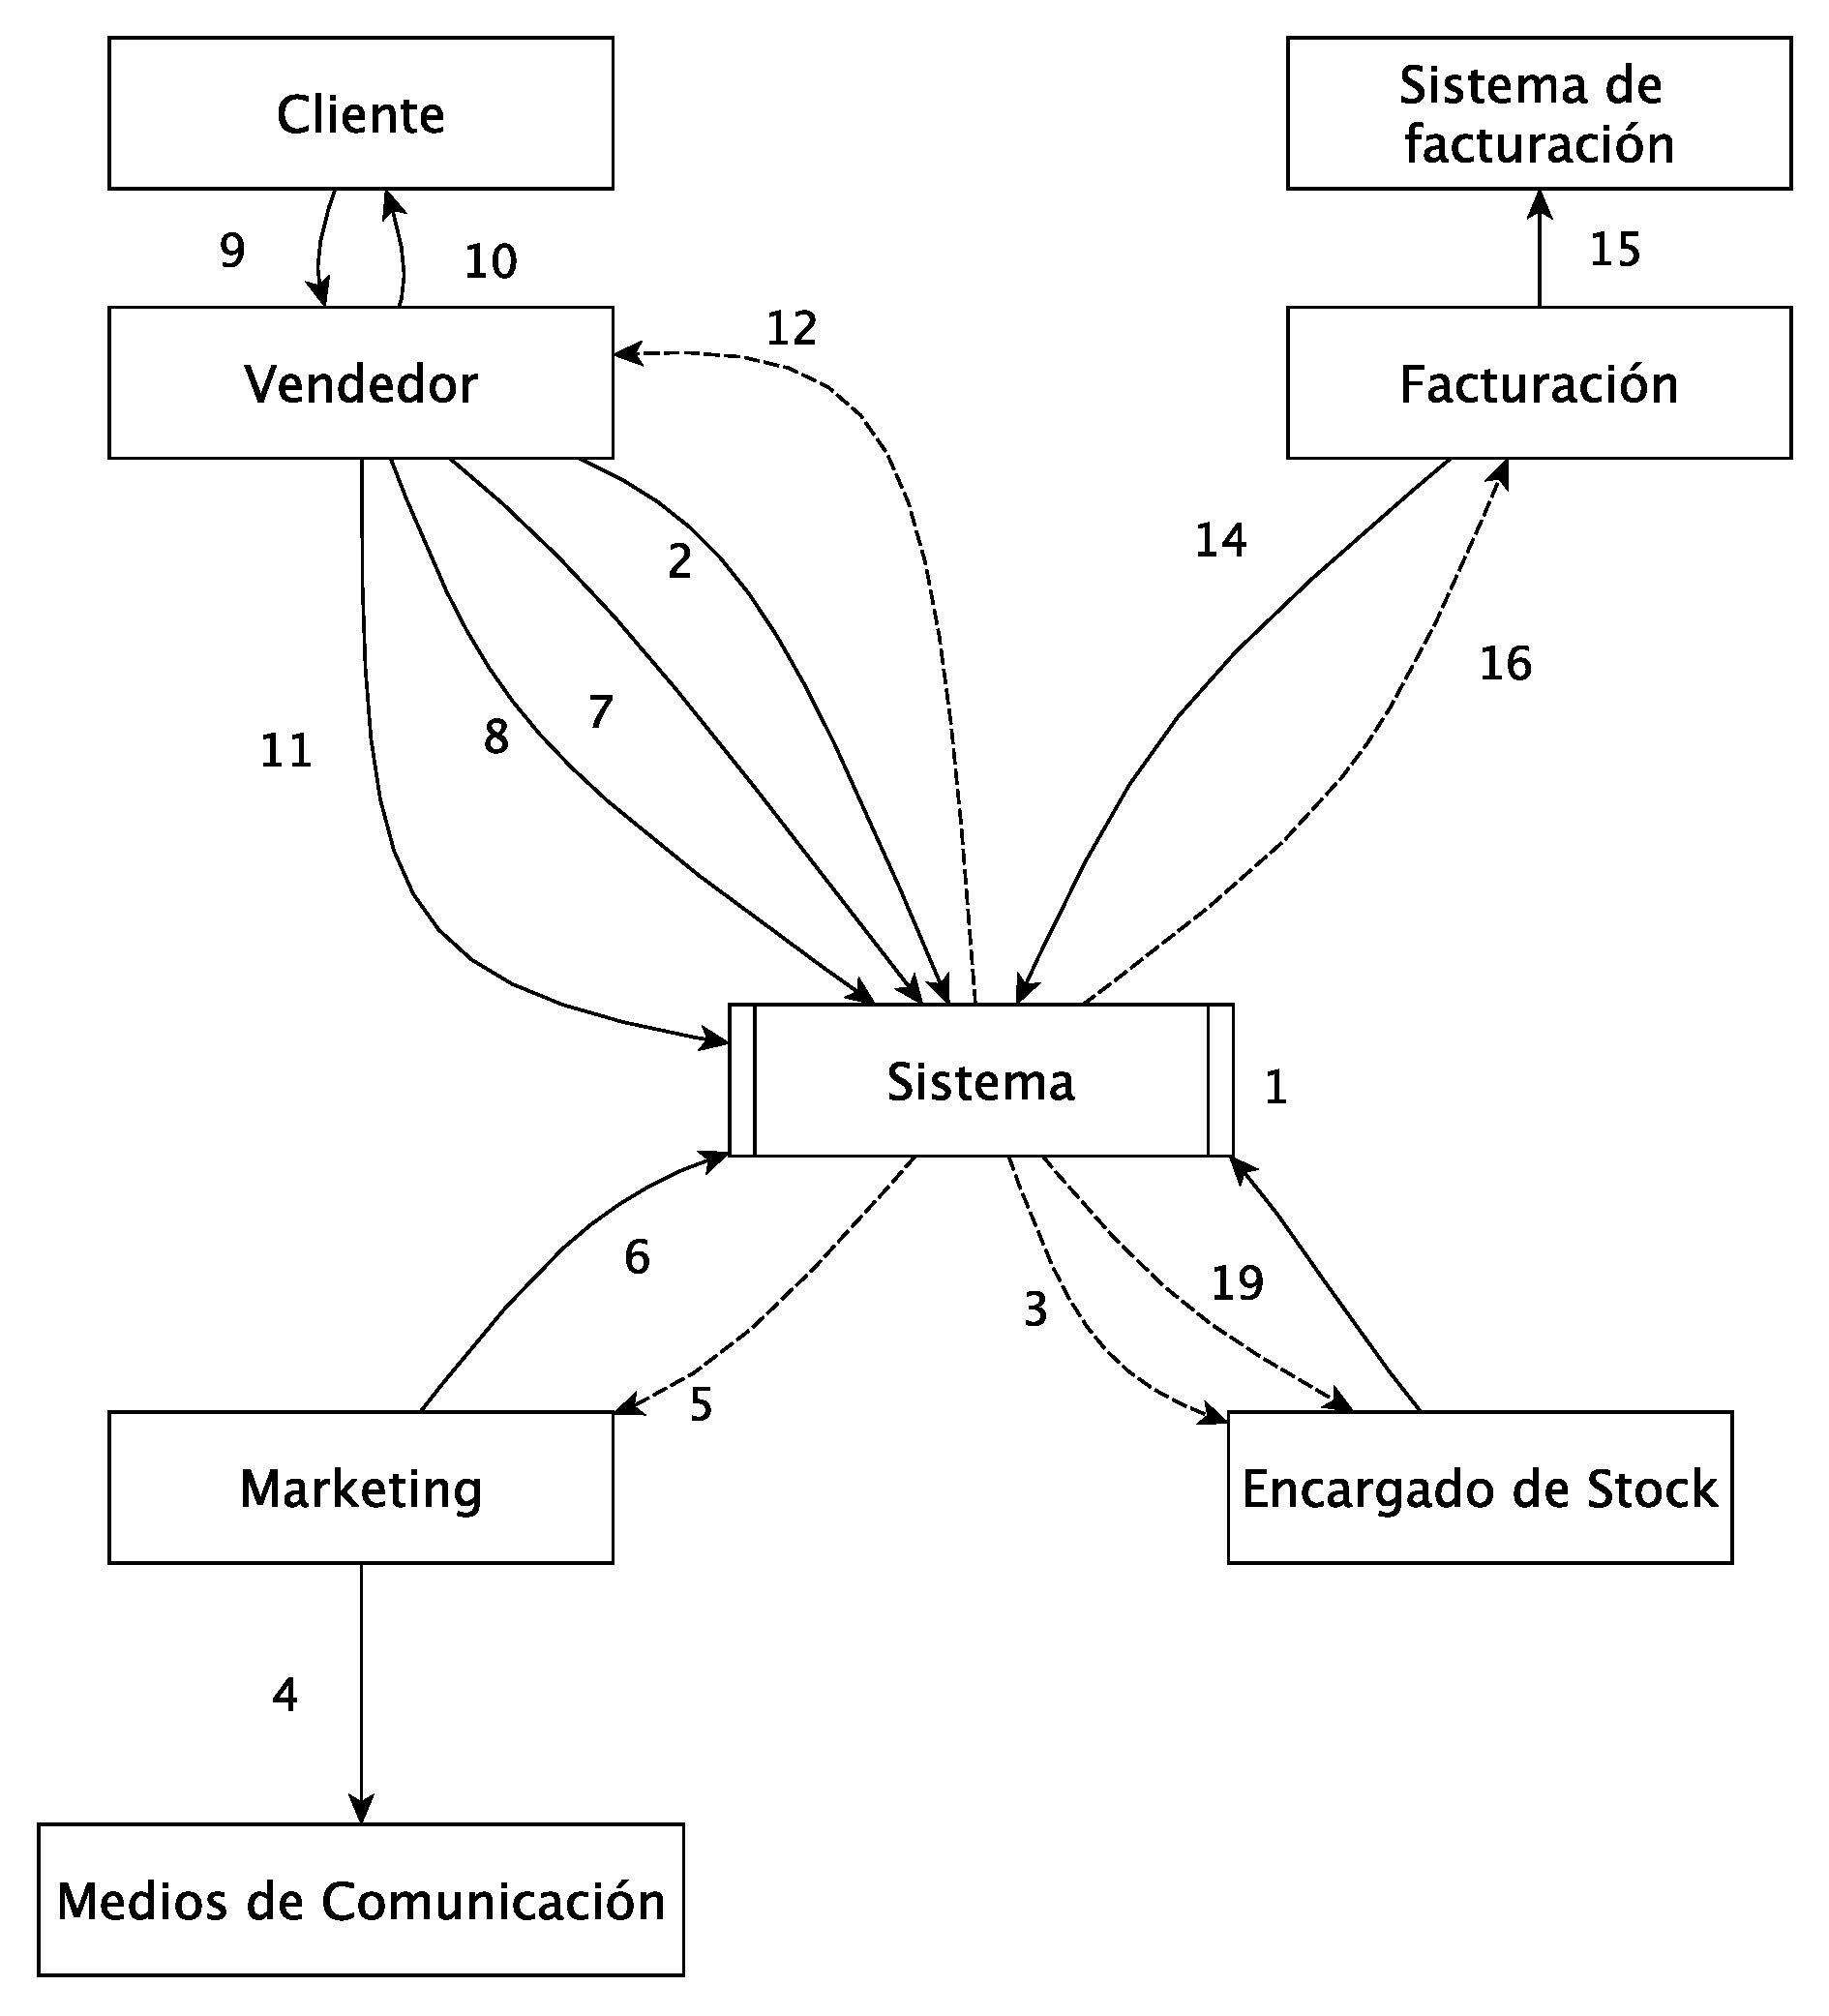
\includegraphics[width=0.5\textwidth]{./imagenes/contexto_2.pdf}
  \caption{Diagrama de Contexto para Sistema de Venta de Celulares (MVP)}
\end{figure}

\subsection{Eventos}

\begin{enumerate}

  \item Ingresar nuevos equipos.
  \item Registrar o cancelar reserva de equipos.
  \item Notificar la confirmación de reserva de equipos.
  \item Monitorear los medios de comunicación.
  \item Notificar stock acumulado.
  \item Dar alta o baja nueva promoción.
  \item Actualizar datos de clientes.
  \item Actualizar promociónes para clientes.
  \item Comunicar necesidades.
  \item Convencer de adquirir promoción.
  \item Seleccionar la promoción adquirida por el cliente.
  \item Confirmar o rechazar promoción por disponibilidad de stock.
  \item Alertar cuando stock está pronto a acabarse.
  \item Confirmar o rechazar venta.
  \item Cargar la venta de los equipos y las líneas.
  \item Notificar venta nueva para ser verificada.

\end{enumerate}

\subsection{Alternativa 2}

En esta segunda opción damos más responsabilidades al sistema para asistir a los 
diferentes departamentos, por ejemplo, realizando un monitoreo de internet para 
favorecer el conocimiento del mercado, o la creación automática de posibles 
promociones basadas en el stock y el análisis del mercado.

\begin{figure}[h!]
  \centering
  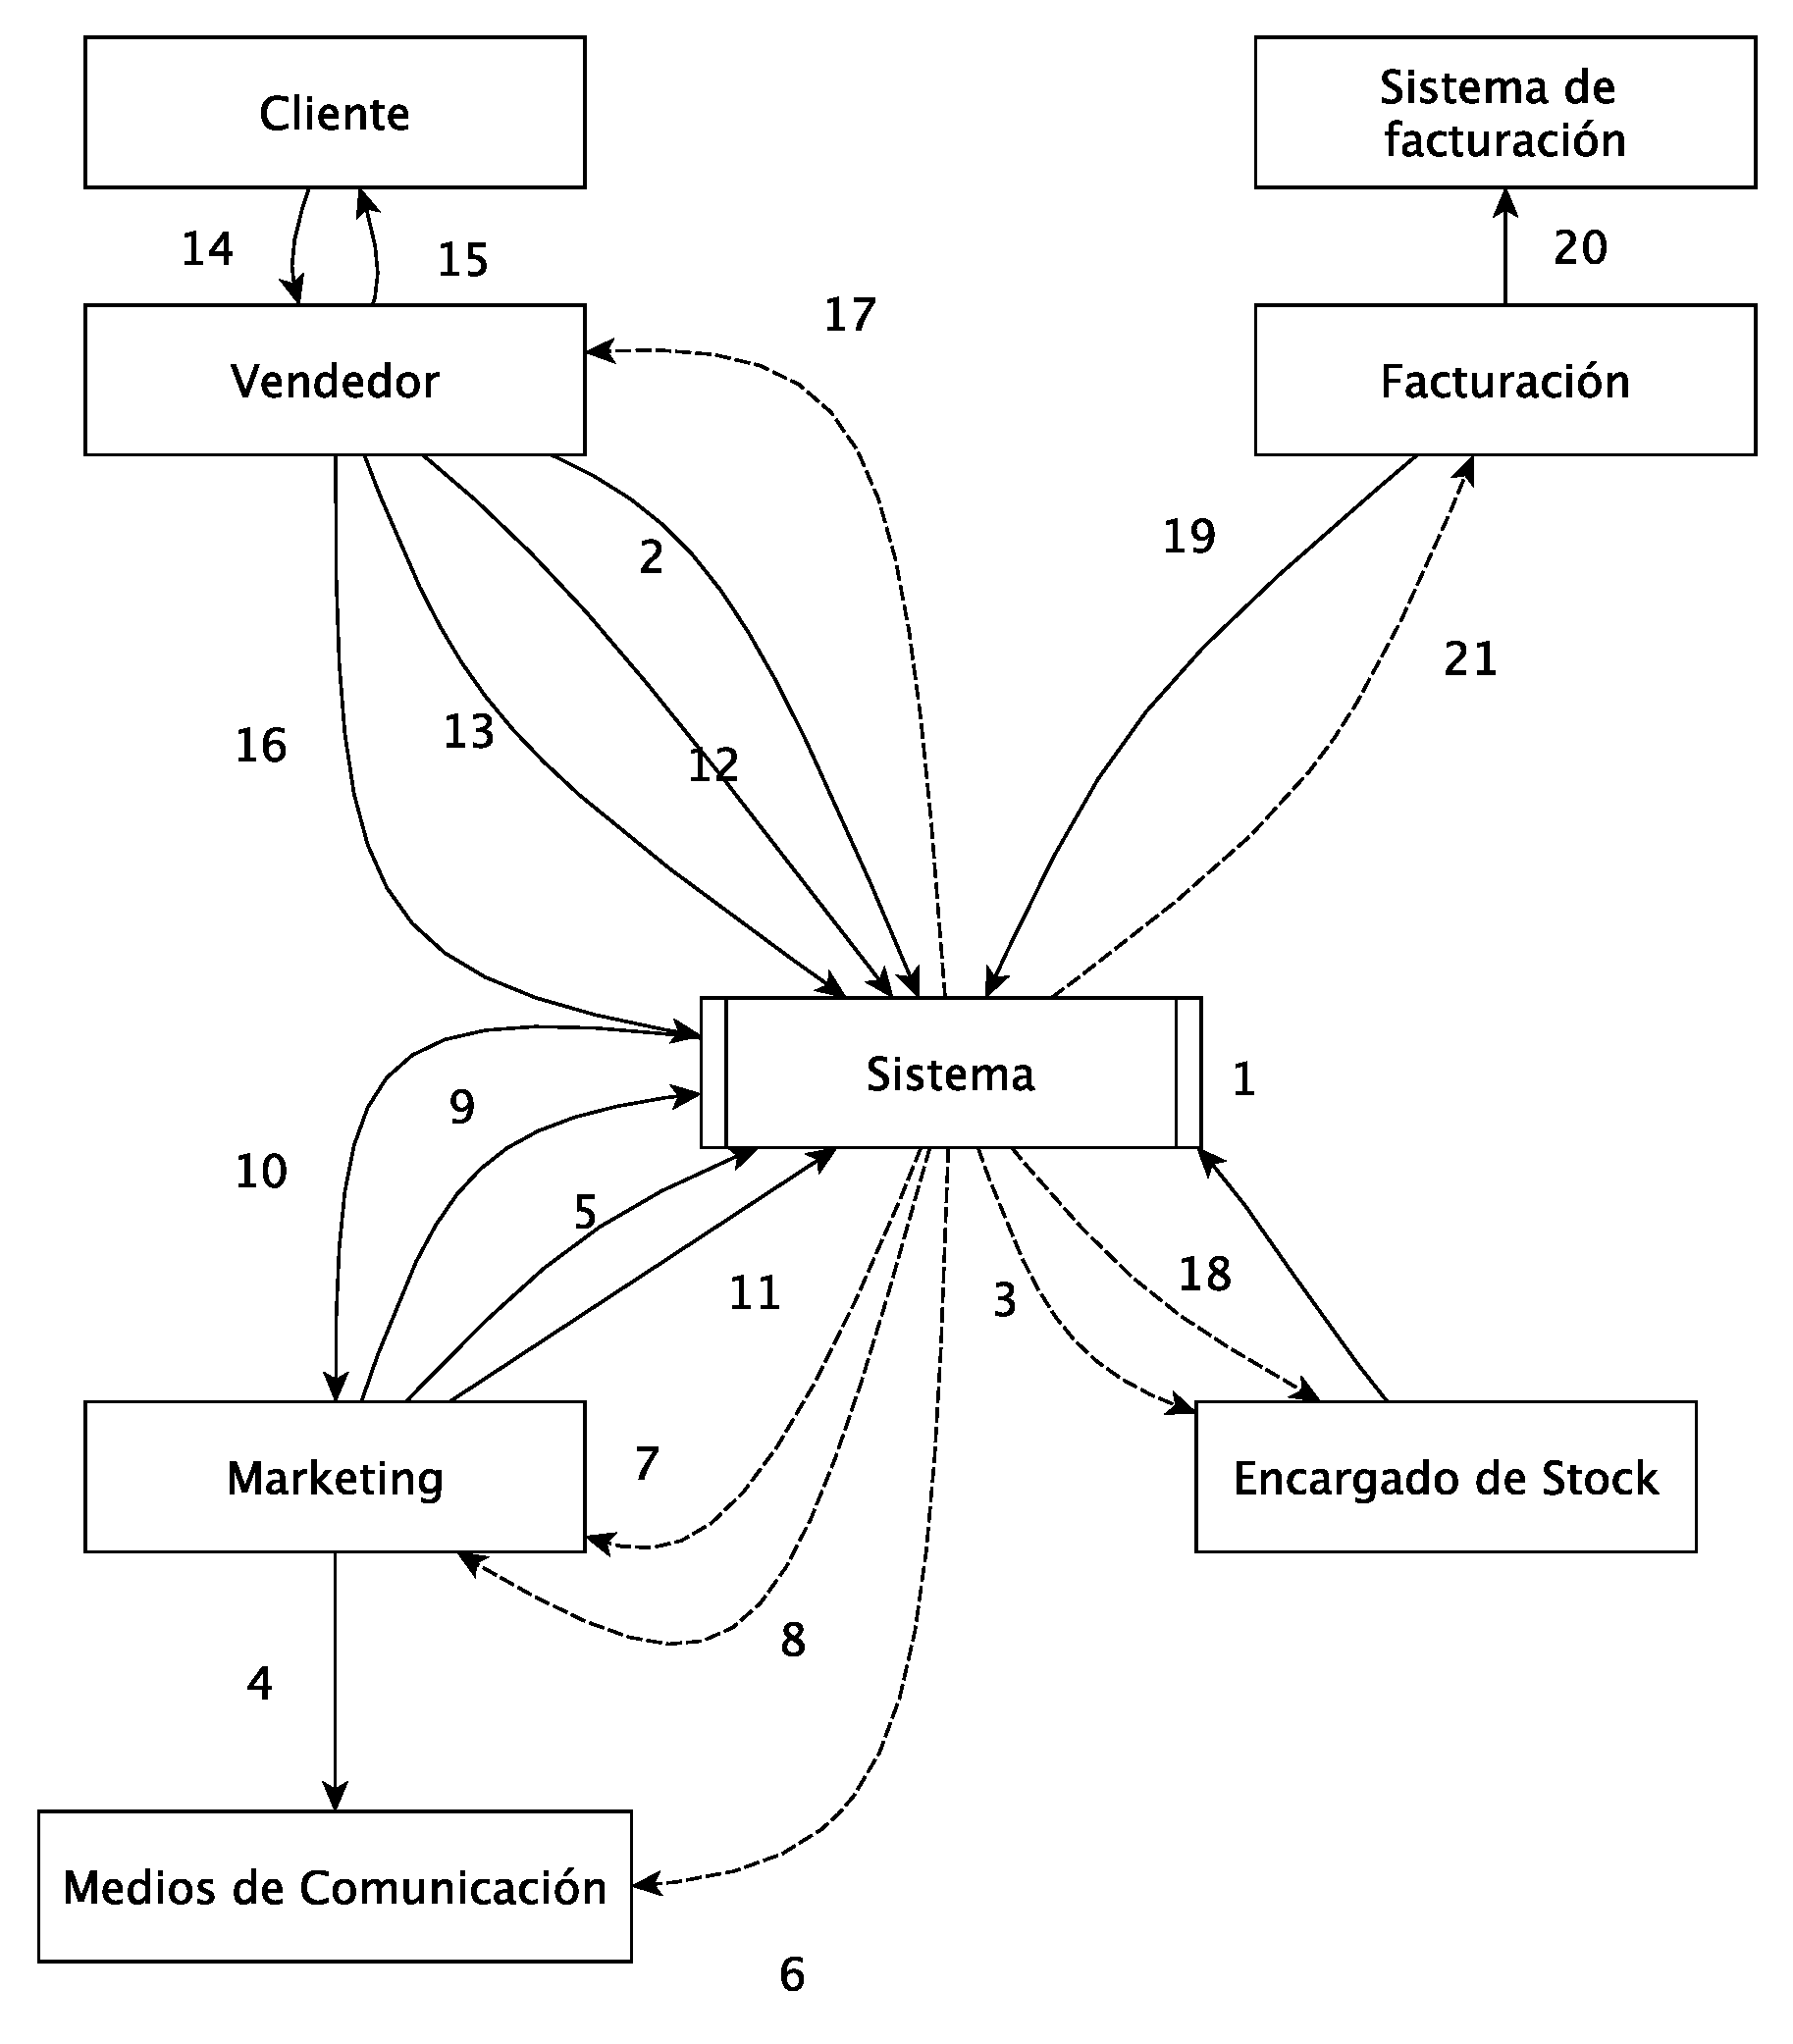
\includegraphics[width=0.5\textwidth]{./imagenes/contexto_1.pdf}
  \caption{Diagrama de Contexto para Sistema de Venta de Celulares}
\end{figure}

\subsection{Eventos}

\begin{enumerate}

  \item Ingresar nuevos equipos.
  \item Registrar o cancelar reserva de equipos.
  \item Notificar la confirmación de reserva de equipos.
  \item Monitorear los medios tradicionales de comunicación.
  \item Seleccionar usuarios y sitos a monitorear.
  \item Monitorear competencia por internet.
  \item Enviar informe de estado del mercado.
  \item Notificar que se creó promoción automáticamente. (vale para mercacdo y stock acumulado)
  \item Validar promoción creada automátiacmente. (vale para mercacdo y stock acumulado)
  \item Notificar stock acumulado.
  \item Dar alta o baja nueva promoción.
  \item Consultar en el momento datos del cliente.
  \item Consultar en el momento promociónes para el cliente.
  \item Comunicar necesidades.
  \item Convencer de adquirir promoción.
  \item Seleccionar la promoción adquirida por el cliente.
  \item Confirmar o rechazar promoción por disponibilidad de stock.
  \item Alertar cuando stock está pronto a acabarse.
  \item Confirmar o rechazar venta.
  \item Cargar la venta de los equipos y las líneas.
  \item Notificar venta nueva para ser verificada.

\end{enumerate}

\clearpage


\section{Diagrama de objetivos}

Para la presentación del diagrama de objetivos decidimos fraccionar el mismo en sus cuatro ramas principales, las cuales componen los aspectos más importantes del diseño del sistema según lo antes descrito. En la figura ~\ref{fig:diagGen} presentamos el nivel superior del diagrama, donde construimos el objetivo principal en base a estos cuatro pilares. Para lograr llevar adelante el sistema que proponemos debemos garantizar, por un lado, poder controlar el stock con precisión y de manera actualizada, registrando ingresos y egresos y, principalmente, evitando problemas de concurrencia entre vendedores actuando al mismo tiempo. Además se deben poder diseñar y cargar con ayuda del software diseñado promociones atractivas para los clientes, no sólo en base a su historia dentro de la empresa sino también en consonancia con el mercado global. Será primordial en el aspecto operativo lograr una venta eficiente y automatizada, donde el vendedor pueda verse desligado de cualquier inconveniente técnico para así poder enfocarse en satisfacer al cliente. Por último, la integración del proceso de venta al sistema informatizado de facturación ayudará a eliminar el esfuerzo y el error humano a la hora de ingresar, contabilizar y facturar las ventas realizadas.

\begin{figure}[h!]
  \centering
  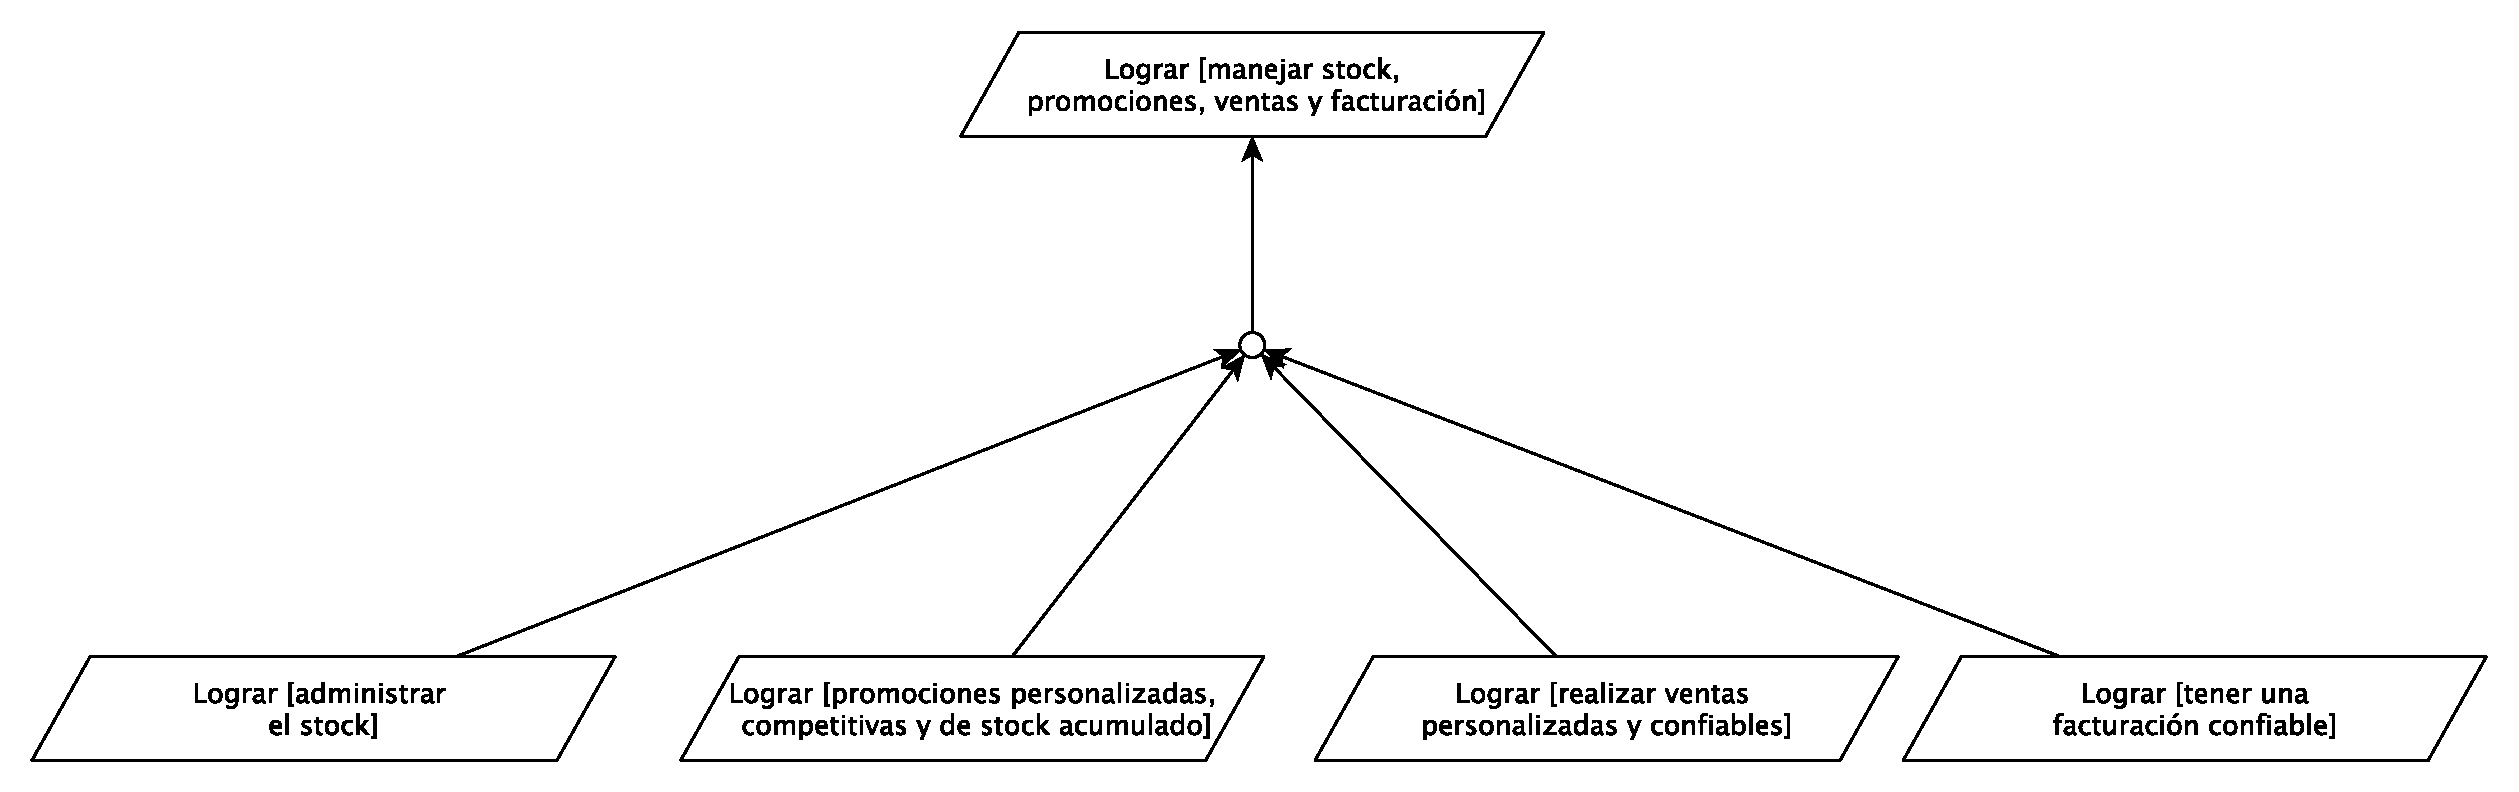
\includegraphics[width=1\textwidth]{./imagenes/general_top.pdf}
  \caption{Diagrama de objetivos - General}
  \label{fig:diagGen}
\end{figure}


\subsection{Rama Stock}

\begin{figure}[h!]
  \centering
  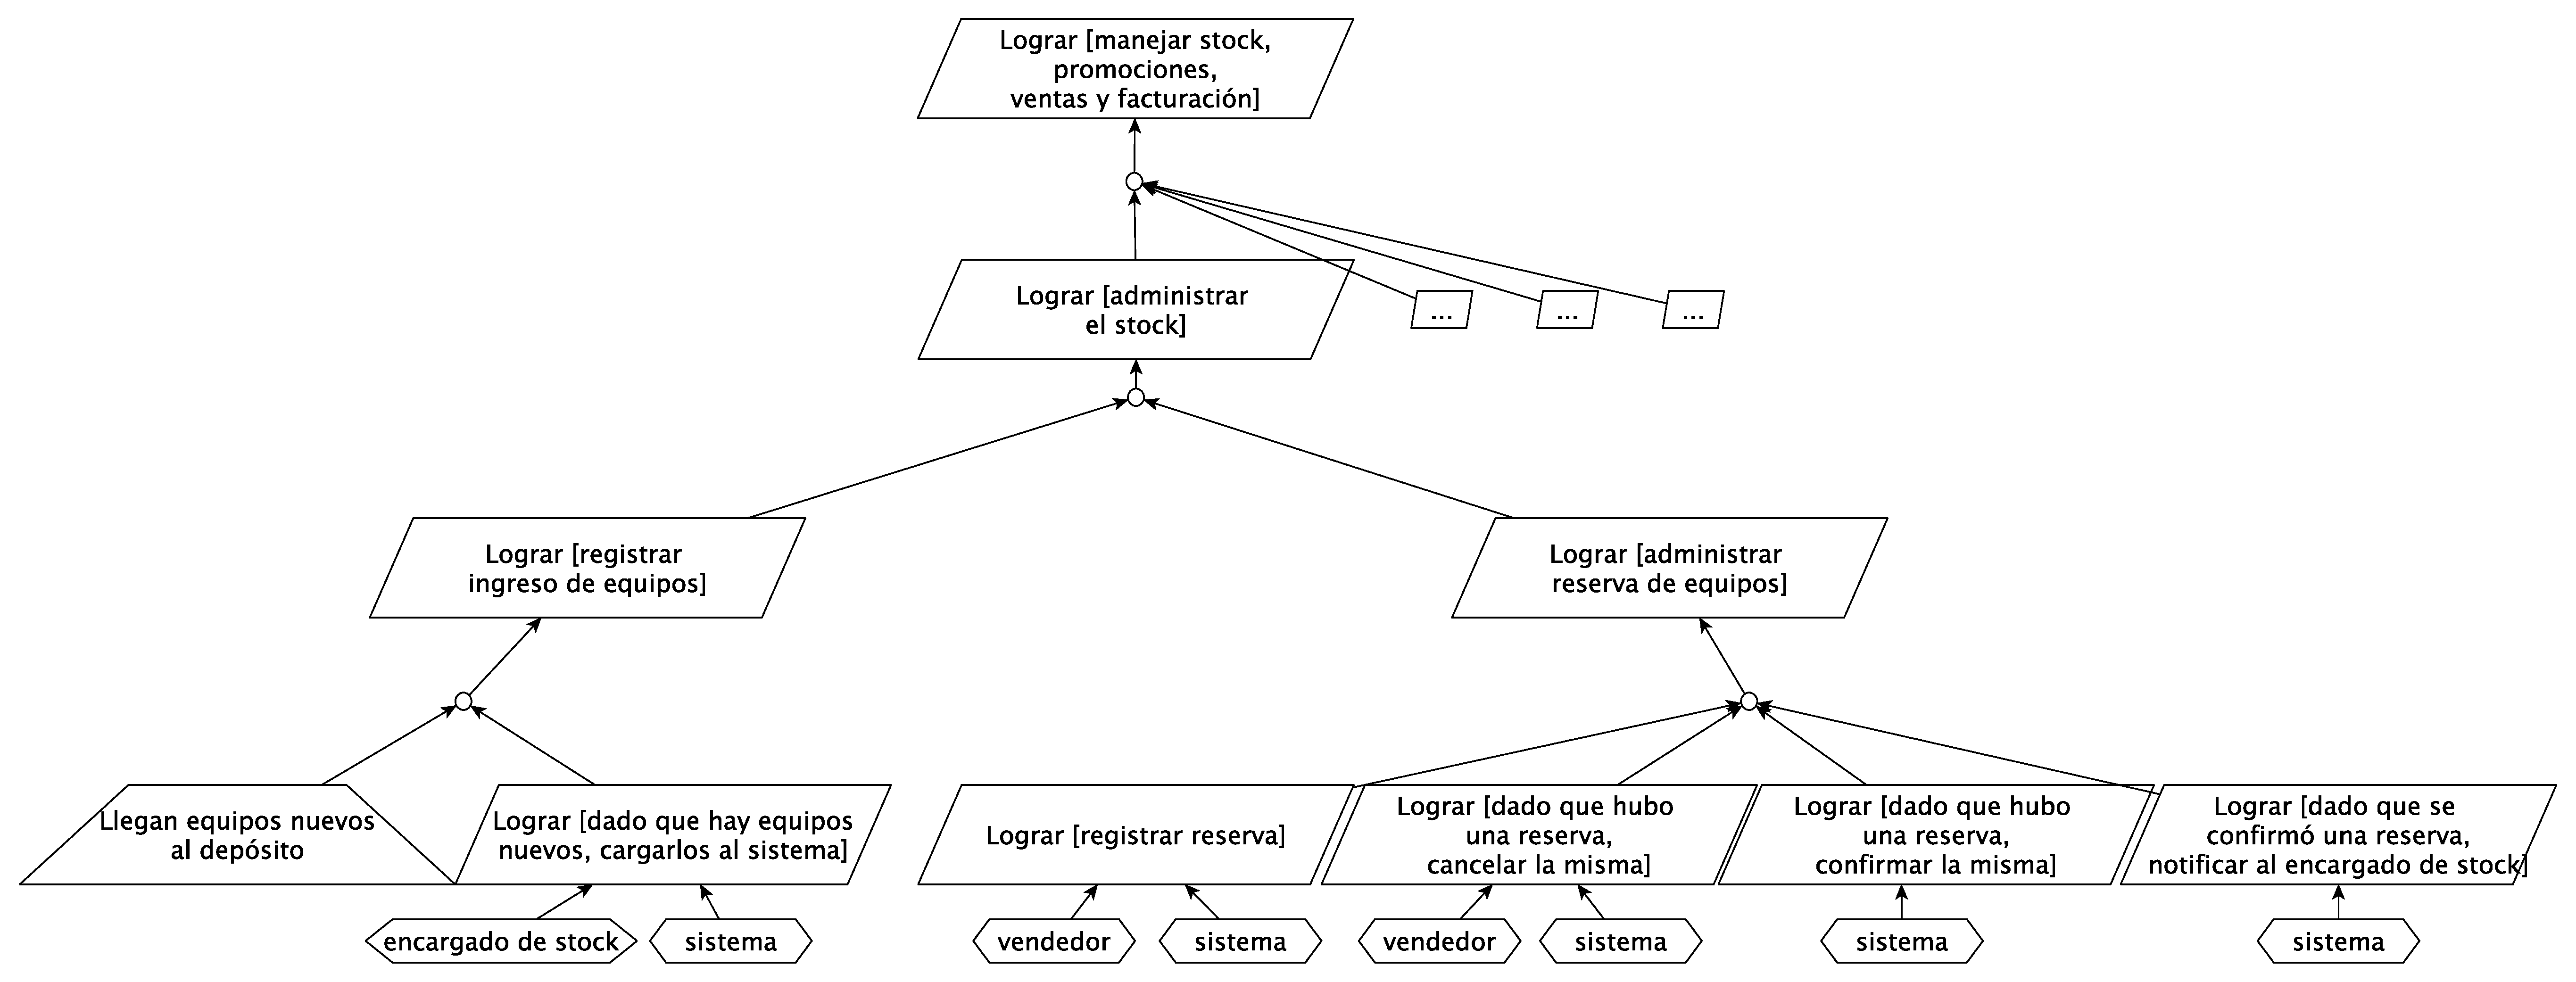
\includegraphics[width=1\textwidth]{./imagenes/stock.pdf}
  \caption{Diagrama de objetivos - Stock}
  \label{fig:diagStock}
\end{figure}

La figura ~\ref{fig:diagStock} presenta la rama de objetivos referente al manejo de stock. La administración del mismo se basa en dos puntos: registrar el ingreso de mercadería nueva y manejar la reserva (y eventual egreso) de los equipos que se vendan. Es importante notar la diferencia entre reserva y venta efectiva (que luego devendrá en egreso del depósito hacia el cliente). Durante la visita del vendedor a un cliente, si éste se decidiera por adquirir una promoción, el vendedor procederá a reservar la misma. Si la reserva le es concedida (ver Rama Ventas), tendrá una ventana de tiempo para confirmar o cancelar la misma. En caso de confirmarla, se le envía una notificación al encargado de stock pero de todas maneras éste deberá aguardar a la notificación de facturación, una vez que la venta haya sido ratificada por el departamento. En caso de cancelación, se restituye la cantidad de stock que se había sacado de circulación al otorgar la reserva para que otros vendedores puedan disponer de esa mercadería. Es importante señalar que la notificación de reserva permite al departamento de stock llevar una cuenta más detallada y controlada del flujo de equipos en sus distintas etapas, a la vez que permite mediante la automatización evitar en un alto grado la disposición errónea de equipos. \\
\indent El control del ingreso de dispositivos móviles es más sencillo y se basa fundamentalmente en la presunción de dominio de que los equipos encargados arriban al depósito en tiempo y forma. Luego, el sistema deberá proveer de una interfaz para que el encargado de stock pueda registrar ese ingreso de manera que esté disponible no sólo para el equipo de ventas sino también para que marketing lance las promociones asociadas con aquellos equipos que sean nuevos y no existieran previamente en el catálogo de la empresa.

\subsubsection{Escenarios}

\begin{itemize}
  \item \textbf{Ingreso de equipos}
    Esteban, el encargado de stock, recibe los nuevos equipos en el depósito y los ingresa en el sistema utilizando la interfaz del mismo.
  \item \textbf{Egreso de equipos}
    Cuando se produce una venta efectiva, el sistema genera una notificación y Esteban debe entregar los equipos al cliente y marcarlos como retirados en el sistema.
\end{itemize}

\subsection{Rama Promociones}

El subárbol de objetivos correspondiente a las promociones fue dividido en dos partes. Satisfacer este aspecto del sistema se basa en cuatro pilares: por un lado lograr promociones parametrizadas y promociones competitivas, objetivos que se exploran en la figura ~\ref{fig:diagProm1}. Por el otro, generar promociones de stock acumulado y mantener actualizado y coherente el catálogo de promociones, metas que se muestran en la figura ~\ref{fig:diagProm2}. En lo que respecta a promociones parametrizadas, este objetivo ataca la necesidad de tener una oferta atractiva para los distintos perfiles de clientes. Gracias a que el sistema lleva cuenta de sus clientes y su historia de consumo, marketing dispone de la información necesaria para crear categorías de clientes en base a la cantidad de líneas que poseen y el dinero que gastan en determinado período y en base a esto generar promociones de acuerdo a los parámetros de estos perfiles. De esta manera, los vendedores podrán optar por consultar promociones a medida del tipo de cliente que visitan de una manera eficiente y rápida.\\
\indent Desde otro enfoque también es importante que las promociones tengan correlación con el estado del mercado y que resulten competitvas respecto de otras empresas de telefonía celular. Para esto deberá conocerse el mercado y luego diseñar ofertas acorde a las conclusiones obtenidas. Aquí se presentan por primera vez alternativas sobre cómo abordar un aspecto del sistema. El alcance del estudio de mercado podrá ser en base a internet o además también en base a los medios de comunicación tradicionales como diarios, revistas, radio, etc. Si bien esta última esfera de comunicación sólo podrá ser analizada manualmente por marketing, una de las alternativas que se ofrece es poder llevar adelante un monitoreo automático de internet (y no manual). A simple vista se puede reflexionar que incorporar al sistema una funcionalidad automática de escaneo del mercado en internet será más costoso y no necesariamente más eficiente que hacerlo de manera manual pero deberá tenerse en cuenta también que permitirá una reacción muy rápida frente a cambios en el mercado para contrarrestar a los competidores. En ese caso, marketing deberá primero definir cierto alcance de la búsqueda como ser sitios, redes sociales, usuarios y canales virtuales de difusión de la empresa. Luego, el sistema procederá a procesar toda esa información y a generar un reporte que será enviado a marketing para su desglose.\\
\indent Una vez que marketing cuenta con el estado de mercado, el objetivo inmediato a satisfacer es la correcta creación de promociones en base a esta información. Nuevamente se ofrecen dos alternativas: la creación manual de las mismas, a cargo de marketing, o una creación automática por parte del sistema pero sujeta a revisión por un agente humano de marketing. Esta vez la disyuntiva es similar, puesto que incorporar un módulo de creación automática de promociones seguramente será más costoso, pero por otro lado si para el estudio de mercado se decidió realizarlo automáticamente, podría impactar en menor medida en el costo del segundo sistema automático dado que podría procesar de manera eficiente el reporte emitido en el primer paso. Además, con el uso cada vez mayor de las redes sociales e internet para la difusión de promociones y ofertas por parte de las companías, a largo plazo podría resultar muy ventajoso y liberador de recursos humanos contar con autogeneración de promociones competitivas.\\
\indent El diseño del sistema no pierde de vista que el objetivo principal de la empresa, en otras palabras, es la rentabilidad. Por eso un objetivo importante que deberá cumplirse es el de la generación de promociones de stock acumulado, es decir, de aquellos conjuntos de equipos que superen cierto número en depósito y sea mejor tratar de despacharlos antes de que se vuelvan obsoletos. Dado que se cumple la administración de stock, el sistema ya cuenta con un monitoreo sumamente actualizado de la mercadería. Según un umbral de alerta definido por el equipo de marketing, el sistema alertará al mismo cuando cierto modele supere ese valor. Otra vez se podrá optar por que marketing diseñe las promociones acordes en este caso de manera manual o que el sistema se encargue y luego marketing las valide. En este caso, la alternativa automatizada no será tan costosa puesto que ya se cuenta con el monitoreo de stock y el tipo de oferta podrá ser parametrizada de antemano por marketing sin mucho problema. De esta manera se ahorrará tiempo y trabajo humano para lograr comercializar de manera efectiva el excedente de mercadería. Por último, es de vital importancia que se pueda regular el catálogo de promociones de manera que se puedan publicar nuevas y no circulen promociones desactualizadas. Todo esto se llevará a cabo mediante una interfaz entre sistema y marketing, lo cual le posibilitará estas acciones al equipo en cuestión.

\subsubsection{Escenarios}

\begin{itemize}
  \item \textbf{Promociones parametrizadas} \\
    Cada trimestre el equipo de Marketing analiza el estado de sus clientes y en base a ello diseña distitnas categorías para ubicarlos. Martín, un empleado de Marketing, consulta en el sistema la cantidad de líneas que posee el cliente 'Los Pollos Hermanos' y el consumo del mismo. El cliente posee 25 líneas de celular de las cuales 10 tienen un plan de datos de internet y el consumo total promedia en \$5000 para el último período. Luego de un trabajo en equipo se diseñan 4 categorías (Clases A,B,C,D), y 'Los Pollos Hermanos' es catalogado como un cliente 'Clase B' dado que la misma abarca clientes con 20-45 líneas y al menos 10 planes de datos, con un consumo promedio mínimo de \$3500. A partir de haber pautado la recategorización de clientes para ese trimestre, el equipo de marketing se abocará el resto del período a diseñar promociones asociadas a las distintas clases según los parámetros de cada una.

  \item \textbf{Promociones competitivas}
  \begin{itemize}
    \item \textbf{Conocer el estado del mercado - Automáticamente} \\
      Martín y el resto del equipo de Marketing ingresan en el sistema las páginas de interés de donde sacar información de la competencia, ya sean redes sociales, blogs, diarios e inclusive las mismas páginas oficiales de las otras empresas. El sistema fue desarrollado para obtener información valiosa de estos sitios utilizando técnicas de DataMining para luego generar un reporte que es enviado al departamento de Marketing. Dado que esta funcionalidad es costosa puesto que debe reacondicionarse constantemente y se utilizan consultores externos para tal fin la herramienta suele estar un poco desactualizada y no siempre genera reportes con datos muy útiles. De todas maneras los empleados de marketing ganan mucho tiempo el cuál invertirán en el diseño concreto de las promociones.
    \item \textbf{Conocer el estado del mercado - Manualmente} \\
      Martín, Manuel, Miriam y Marisol revisan periodicamente las redes sociales, blogs, diarios y páginas de la competencia para elaborar el reporte que necesita Marketing para poder diseñar promociones competitivas. Es un trabajo arduo y que requiere de un análisis minucioso de todas las fuentes de información, pero por lo general una vez terminado las conclusiones resultan muy útiles para diseñar promociones originales y rentables.
    \item \textbf{Conocer el estado del mercado - Híbrido} \\
      Manuel y Marisol revisan perioóicamente las páginas de la competencia y blogs, mientras que a la par el sistema obtiene información de las redes sociales seleccionadas en tiempo real. Este análisis automático es menos costoso porque su espectro de búsqueda es reducido y acotado siempre a las mismas redes sociales. Es más dinámico, se puede realizar con más frecuencia y de ambos mecanismos los empleados elaboran un reporte final que será utilizado luego para ponderar las promociones competitivas a confeccionar.
  \end{itemize}

  \begin{itemize}
    \item \textbf{Crear promociones en base a reporte - Manualmente} \\
      Miriam y Marisol analizan el reporte sobre el estado del mercado, discuten y diseñan nuevas promociones.
    \item \textbf{Crear promociones en base a reporte - Automáticamente + Verificación} \\
      Miriam y Marisol deben introducir manualmente algunos datos clave de el reporte que generaron manualmente para que el sistema diseñe promociones competitivas similares a las recolectadas por los empleados. Esto es nuevamente tedioso, ya que tienen que reajustar la información recabada para poder utilizarla como punto de entrada a la función autogeneradora de promociones.\\
      En cambio, dado un reporte de mercado autogenerado, el mismo habrá sido configurado para que sus datos de salida sean válidos como entrada al sistema autogenerador de promociones, con lo cual se realiza todo en un mismo flujo de trabajo lo que implica una gran ventaja en términos de tiempo y esfuerzo para los empleados de marketing. No obstante la calidad del resultado estará sujeta a la precisión del reporte de mercado ingresado.\\
Finalmente, en ambos casos, el equipo de Marketing es notificado al finalizar el diseño automático de promociones para encargarse de su verificación.
  \end{itemize}

  \item \textbf{Promociones de Stock acumulado} \\
    El sistema mantiene actualizado el inventario de la empresa y registro de los movimientos de cada equipo. Cuando el sistema detecta que bajan las ventas de determinados equipos o se empieza a acumular en el depósito, éste notifica al departamento de Marketing para crear promociones con estos equipos.
  \begin{itemize}
    \item \textbf{Crear promociones - Manualmente} \\
      Manuel y Miriam detectan que el iPhone 4, recientemente salido al mercado, no está registrando las ventas esperadas, y al tiempo se alarman al recibir un llamado del encargado de stock debido a que hay un excedente inusual de este producto. Al mismo tiempo observan en las noticias que ese modelo había salido de fábrica con un problema en su antena, lo que generaba problemas con la señal y debido a esto su fama iba de mal en peor. Para poder disponer de las unidades en depósito y no generar pérdidas a la empresa, ambos empleados deciden diseñar una promoción especial donde ofrecen un $2x1$ de ese modelo con plan de datos bonificado por 6 meses.
    \item \textbf{Crear promociones - Automaticamente + Verificación} \\
      El equipo de Marketing ha configurado un umbral de alarma de 600 unidades en depósito durante dos semanas seguidas para cualquier modelo de celular. Al generarse una de las notificaciones del sistema, el mismo captura este alerta y calcula, en base a ciertas reglas de negocio predefinidas por Marketing, distintas promociones de stock acumulado automáticas donde se buscará poder reactivar la venta de ese modelo con la mejor rentabilidad posible. Manuel, en su avidez por traerle a la empresa el mayor rédito posible, realiza una carga de parámetros de negocios un tanto errónea por lo que, cuando el iPhone 4s deja de ser requerido debido a sus problemas técnicos, el sistema crea una promo donde ofrece 1 (una) unidad por el precio de 3 (tres). Afortunadamente Miriam realiza su trabajo de verificación, detecta lo absurdo de la propuesta y la corrige según un criterio más sensato antes de que se publique a la flota de vendedores.
  \end{itemize}

  \item \textbf{Actualizar la lista de promociones vigentes} \\
    Marisol tiene pendientes 5 promociones navideñas que ha realizado con su equipo, 2 de las cuales fueron autogeneradas y luego verificadas, y el resto diseñadas manualmente. Procede a cargarlas y a publicarlas para que el resto de los vendedores puedan verlas, pero pronto detecta que una de las diseñadas automáticamente no fue correctamente verificada y está mal formulada. Rápidamente la elimina y actualiza el catálogo para que los vendedores (bajo el sistema con internet) puedan recibir en tiempo real la información correcta. Al mes siguiente, Marisol misma es la encargada de retirar las promociones que había cargado dado que la época de navidad ha pasado. 
\end{itemize}

\clearpage

\begin{figure}[h!]
  \centering
  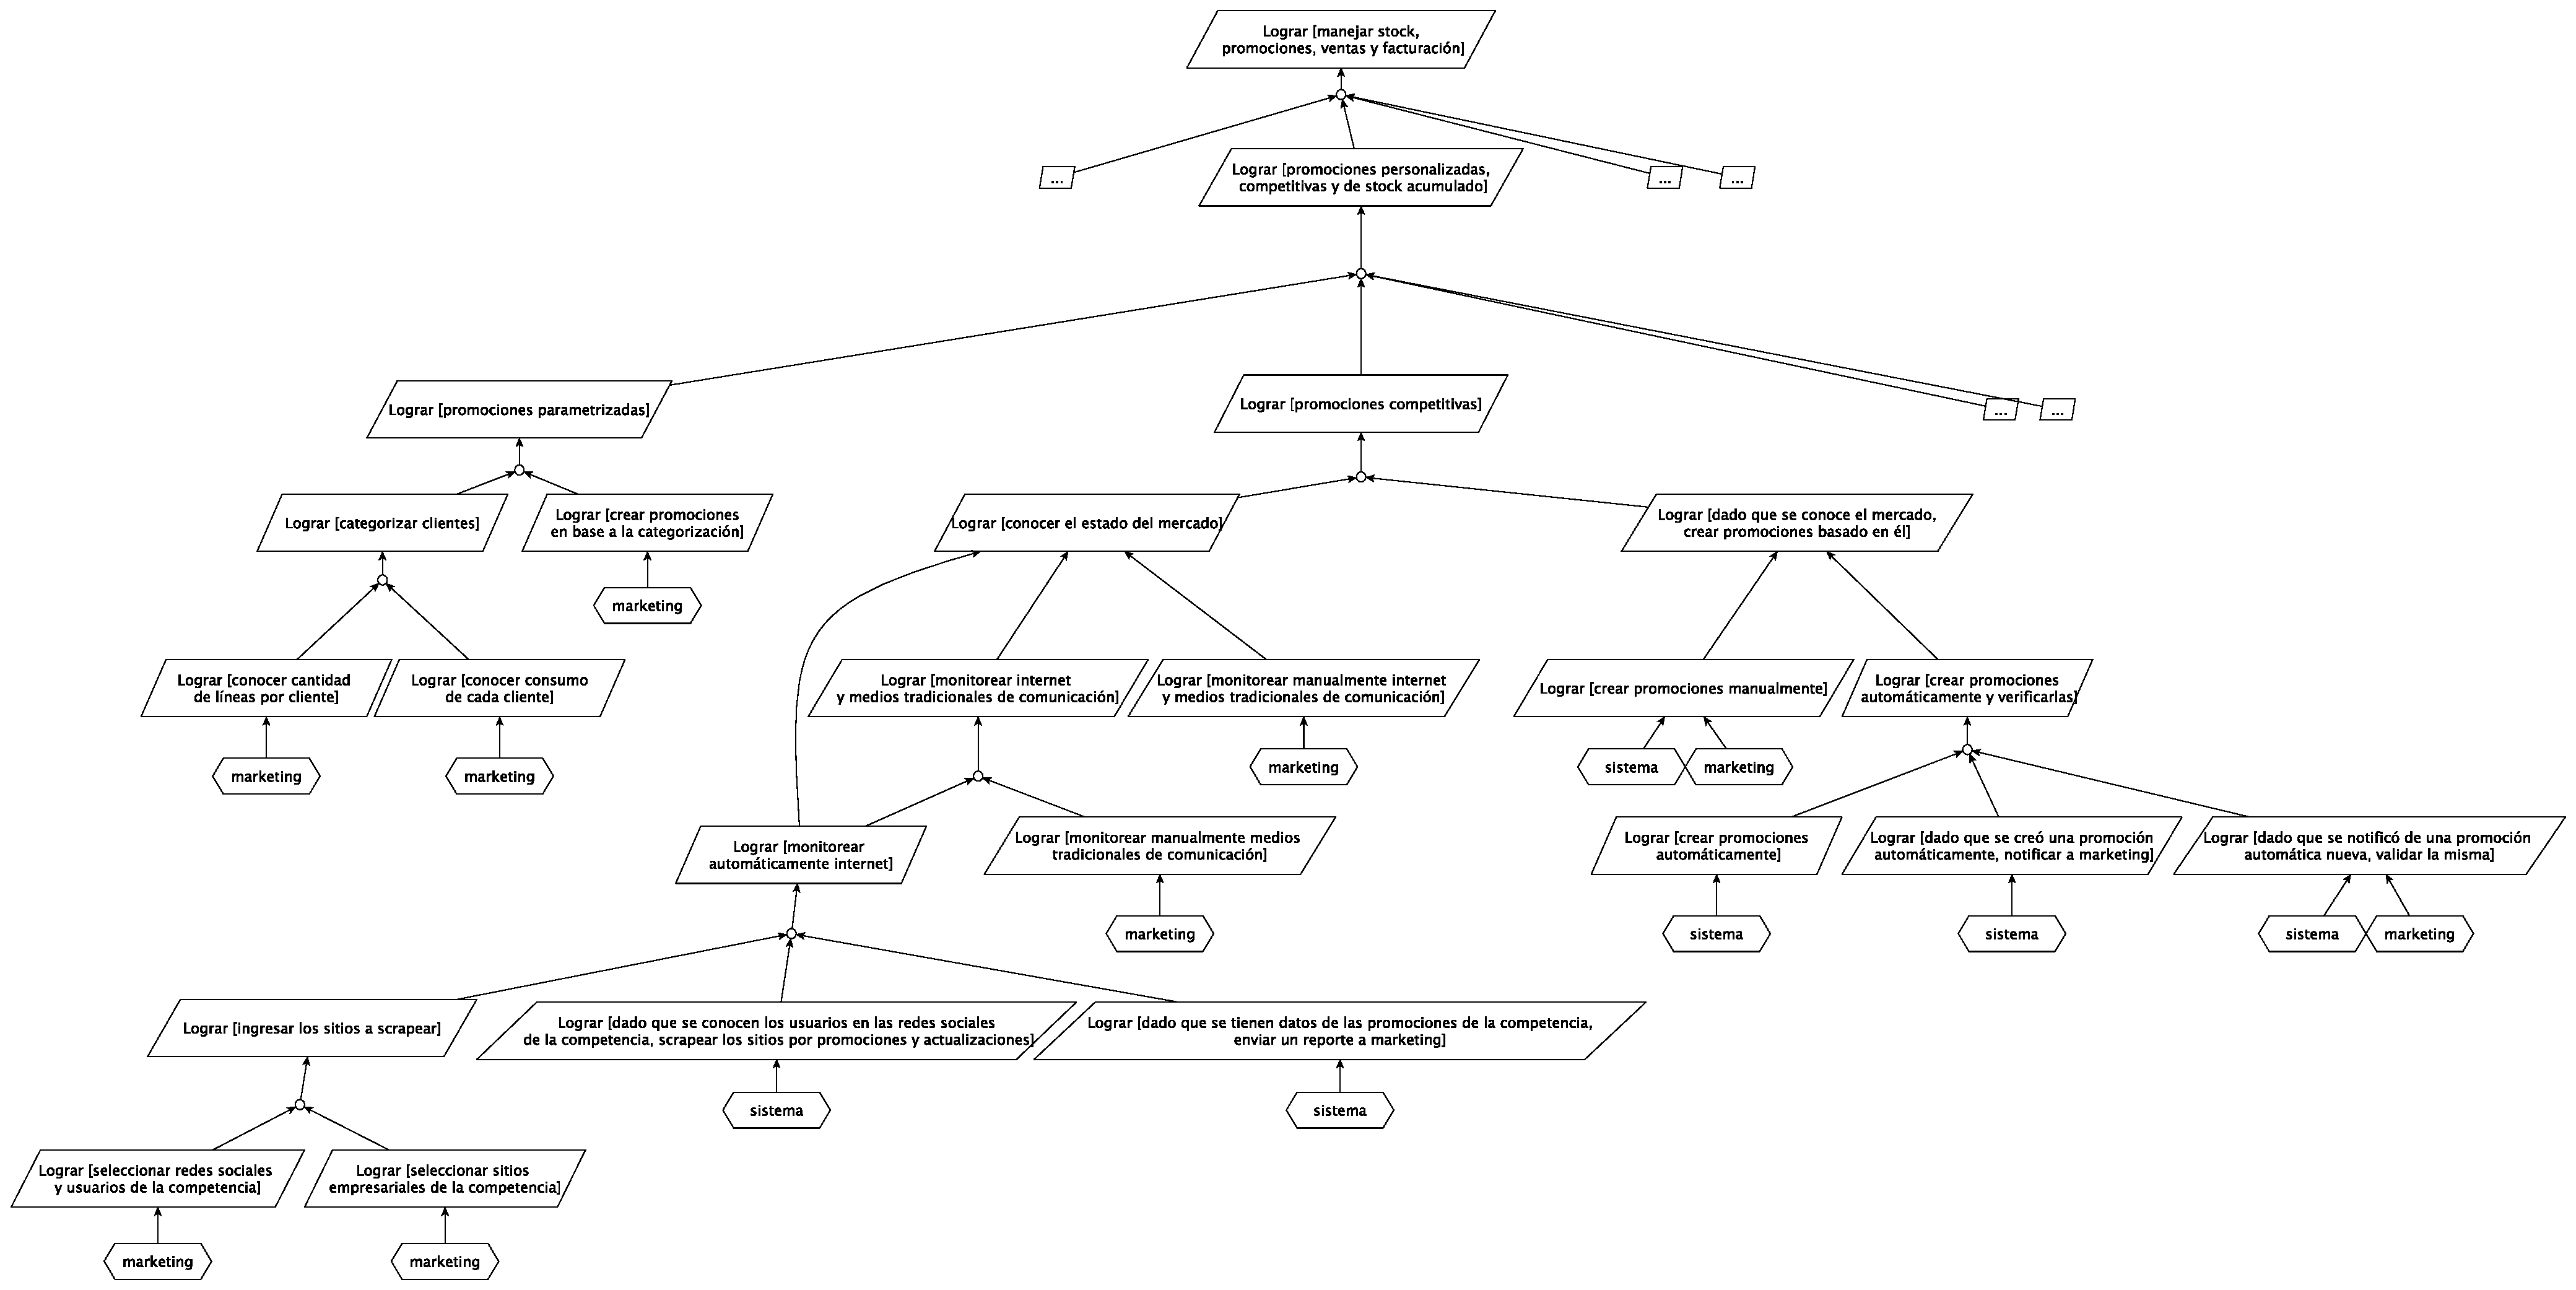
\includegraphics[width=1.5\textwidth, angle=90]{./imagenes/promociones_1.pdf}
  \caption{Diagrama de objetivos - Promociones (parte 1)}
  \label{fig:diagProm1}
\end{figure}

\clearpage


\begin{figure}[h!]
  \centering
  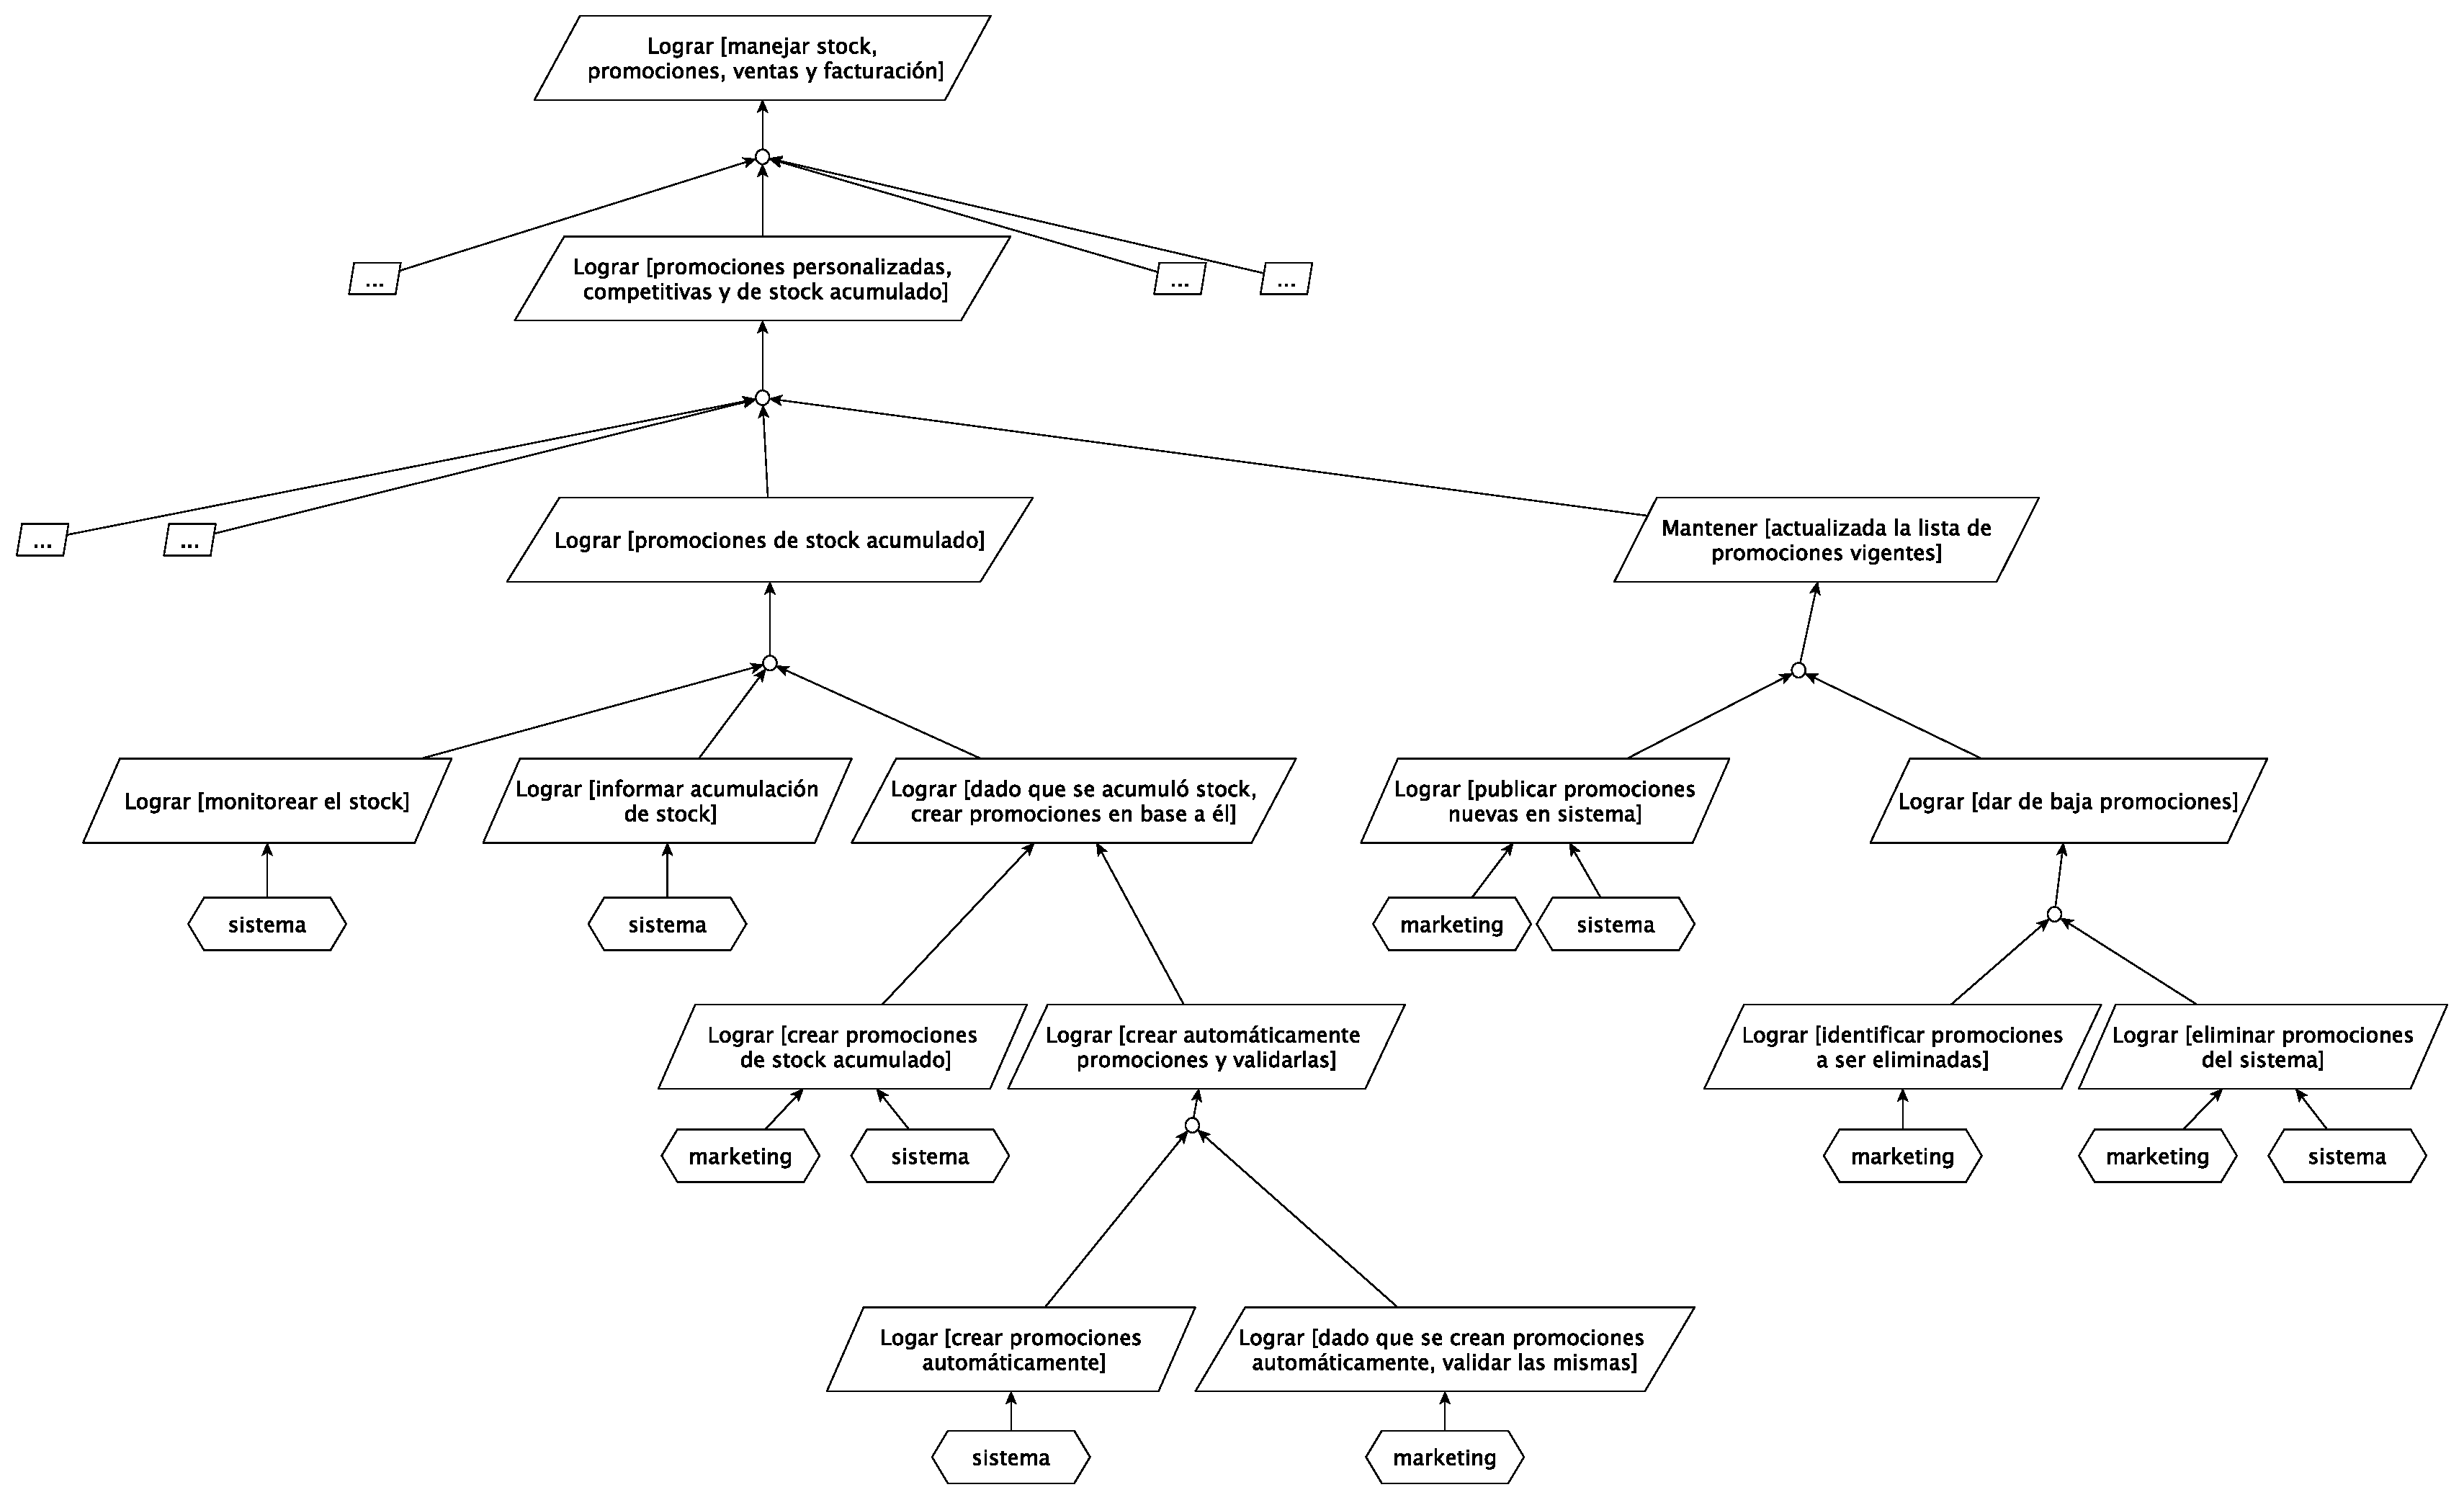
\includegraphics[width=1.3\textwidth, angle=90]{./imagenes/promociones_2.pdf}
  \caption{Diagrama de objetivos - Promociones (parte 2)}
  \label{fig:diagProm2}
\end{figure}

\clearpage

\subsection{Rama Ventas}

Nuestro sistema tiene como objetivo lograr realizar ventas personalizadas y confiables. Para lograr esto tenemos 6 objetivos a cumplir. A saber:
\begin{enumerate}
  \item Conocer los datos del cliente.
  \item Conocer las promociones disponibles para el mismo.
  \item Adaptar las promociones a necesidades particulares.
  \item Convencer al cliente de comprar una promoción.
  \item Reservar la misma.
  \item Confirmar la compra.
\end{enumerate}

\indent Para conocer los datos del cliente se debe averiguar, por un lado, la cantidad de líneas y la facturación mensual que posee en nuestra empresa, y por otro, las necesidades del mismo.\\
\indent El primer par de objetivos se puede obtener de dos formas: manteniendo los datos de los clientes a visitar en el dispositivo móvil del vendedor, actualizando diáriamente el dispositivo, o dándole la posibilidad de consultar los datos del cliente en el momento de forma inalámbrica.

\indent Asumiendo que ya conocemos los datos del cliente, queremos conocer que promociones tiene nuestra empresa para él. De manera similar a la anterior, tenemos la opción offline y la online. La offline consiste en mantener las promociones para los clientes a visitar en el dispositivo móvil del vendedor, actualizándo diariamente los datos de las promociones en el mismo. La opción online se basa en tener disponible las promociones para el cliente de manera inalámbrica. Un objetivo blando que nos planteamos es el de contar con las últimas promociones realizadas por marketing. La opción offline contribuye un poco a lograr esto, mientras que la online contribuye bastante, por poder tener disponibles las últimas generadas en el mismo día.\\
\\

\indent Nuestro sistema de ventas debe poder, luego que se adaptaron las promociones disponibles para el cliente a sus necesidades particulares y que se lo convenció de comprar una de las mismas, reservar una promoción.\\
\indent Para cumplir este objetivo se deben dar tres cosas:
\begin{enumerate}
  \item Se debe poder ingresar la promoción elegida, para lo cual necesitamos seleccionarla de una lista y enviarla al servidor.
  \item Se debe poder, dado que sucedió lo anteriormente dicho, comprobar la disponibilidad del stock para reservarla, manteniendo una conexión con el servidor (detalles sobre este objetivo más adelante).
  \item Se debe poder mantener actualizado el stock, dado que hubo disponibilidad para la reserva. Para esto debemos descontar el stock reservado y notificar al encargado si el stock está pronto a terminarse.
\end{enumerate}

\indent Por último, asumiendo que se cumplió lo anteriormente descripto, debemos lograr confirmar la compra. Esto se consigue logrando ingresar los datos del cliente necesarios para comprar, y enviándolos al servidor manteniendo la comunicación con el mismo.\\
\indent Hay dos formas de ingresar los datos del cliente necesarios para comprar: Se puede obtener los datos leyendo el código QR provisto por la AFIP de Cambodia, o se puede completar el formulario de facturación. Ambos contribuyen a disminuir el error humano, el primero por no necesitar de ninguna interacción al ingresar datos, y el segundo si bien requiere completar un formulario, es menos propenso a error que copiar datos de una tabla donde es fácil confundir las filas.\\

\indent El objetivo común que describimos como ``mantener comunicación con el servidor'' influye en cuatro objetivos blandos:
\begin{enumerate}
  \item Tener mayor performance.
  \item Tener disponible el servicio el mayor tiempo posible.
  \item Tener una comunicación segura.
  \item Reducir el costo de desarrollo y mantenimiento.
\end{enumerate}

Dicho objetivo común se puede lograr de dos maneras: mediante internet móvil o mediante envío y recepción de SMS. La forma en la que lo hace, es la siguiente:
\begin{itemize}
  \item Internet móvil: ayuda en gran parte al cumplimiento de los objetivos blandos 1 y 3, gracias a su velocidad y capacidad de encriptación. Ayuda también un poco al objetivo 4, y no consigue cumplir muy bien el 2, por lo planteado en el enunciado (el servicio es propenso a caerse).

  \item Envío y recepción de SMS: es una opción mala para el objetivo blando número 3, ya que no existe encriptación, y también para el objetivo 4. Es un poco peor que la alternativa de Internet móvil para el objetivo 1, y ayuda a cumplir el objetivo 2, ya que generalmente es un servicio que está disponible siempre.
\end{itemize}

\indent Para lograr comunicarse a través de internet, asumimos que el dispositivo móvil del vendedor tiene conexión a internet, y el mismo debe lograr enviar un pedido y recibir una respuesta. Para poder comunicarse a través de SMS, asumimos que el dispositivo cuenta con un chip GSM para conectarse a la red, y que nuevamente puede por este medio enviar un pedido y recibir una respuesta.

\subsubsection{Escenarios}

\begin{itemize}
  \item \textbf{Conocer los datos del cliente} \\
    Víctor, vendedor audaz, entra en las oficinas de Clelia \& Company.
    Luego de la introducción comienza con su trabajo consultando al sistema
    la cantidad de líneas y facturación del cliente, así como también su categoría. Esto lo obtiene en tiempo real a través de internet, que por fortuna en los primeros minutos de la reunión funciona correctamente. Por otro lado le consulta al cliente cuán satisfecho está con el servicio, si necesita ampliar su red de telefonía, necesita más planes de datos, o por el contrario reducir costos, actualizar equipos, etc.\\
	Remo Erdosain, por otro lado, acude por la mañana a la central de la empresa de telefonía para que carguen en su dispositvo la última base de clientes y promociones, para luego embarcarse a visitar a su primer cliente. Dado que el servicio de internet sufre caídas permanentemente y no desea pasar más situaciones incómodas ante sus clientes, Remo ha pedido a la empresa realizar su trabajo mediante otro sistema de comunicación que ofrezca mejor cobertura y permanencia de servicio. Es así como llega a las oficinas de la 'Industrias Gobias' para encontrarse con su primer cliente.\\

  \item \textbf{Conocer y Adaptar las promociones para el cliente / Reservar una promoción} \\
    Victor, luego de conocer las necesidades del cliente, utiliza su dispositivo para obtener las distintas promociones disponibles. Dado que ha identificado al consumidor, el sistema trae las promociones acorde a su categoría, además de otras especiales muy competitivas, y algunas otras al azar. Víctor puede ajustar esta búsqueda introduciendo la información recabada en la entrevista para poder precisar mejor de qué dispone para satisfacer al cliente. Por mala fortuna, durante esta consulta de promociones el servicio de internet tiene un breve corte lo cual fuerza a Víctor a desplegar sus dotes comerciales para distraer al cliente y evitar mostrar la debilidad de su servicio. Una vez retornada la conexión de internet móvil, Víctor selecciona las 3 promociones que mejor se ajustan a lo expresado por Clelia y, técnicas persuasivas mediante, lo logra convencer de optar por una. Continuando con la mala fortuna, al querer realizar la reserva el sistema le informa al vendedor que ya no quedan suficientes unidades disponibles para satisfacer el pedido, con lo cual Víctor debe volver a la carga para lograr convencer al cliente de que opte por la segunda opción. Dado que el cliente se muestra un tanto reacio ante la no disponibilidad de su primera elección, Víctor se toma la licencia de modificar levemente la promoción cargada por Marketing para personalizarla y volverla más atractiva económicamente hacia el cliente. Esto da buenos resultados, con lo cual Víctor logra venderle esta promoción modificada que no presenta problemas de stock.\\
Remo Erdosain acude tranquilo a su primer cliente confiando en que esta vez no tendrá problemas de conectividad con internet con el nuevo sistema. Habiéndo consultado los datos del mismo procede a listar las promociones disponibles del día. Lamentablemente, Remo no posee el catálogo actualizado puesto que lo cargó en la mañana y Marisol, de Marketing, decidió remover en el interín de la mañana algunas promociones que, debido a la inflación, habían quedado demasiado desactualizadas. Remo, desconociendo este cambio, logra convencer al cliente de que opte por una de estas promociones ya obsoletas, pero a la hora de realizar la reserva el sistema le comunica que esa promoción ya no está disponible. Finalmente el cliente decide no contratar una nueva promoción, por lo que Remo pasa a su segundo visitado del día. Nuevamente el panorama parece estar destinado al fracaso puesto que Remo elige una promoción cuyo stock acaba de ser agotado por otra vendedora - Virginia - en otra punta de la ciudad (aunque él no lo sabe). Remo procede a realizar la reserva pero nota que la confirmación de la misma demora más de lo usual, y en su interior reflexiona que probablemente sea producto de que la comunicación con la central se realiza por SMS y no por internet. En el mismo momento, el cliente de Virginia cambia repentinamente de opinión y puesto que la vendedora aún no había confirmado la venta logra cancelarla, lo cual restituye las unidades de stock antes inhabilitadas. Dado que el SMS detrás de esta cancelación llega antes que el de Remo, éste nunca se entera de que al querer reservar la promoción no había stock, y gracias a la tardanza del mensaje evita volver a pasar por una situación desalentadora y logra concretar su venta.

  \item \textbf{Confirmar la venta} \\
	Para ratificar la reserva y así enviar la venta a facturación, Víctor debe ingresar manualmente los datos de facturación del cliente como tarjeta de crédito, datos de AFIP, y además Clelia puede optar por elegir algún prefijo para las nuevas líneas de celulares. Víctor tiene mucho cuidado al ingresar estos datos porque sabe, por experiencias pasadas, que un error en el ingreso de los datos puede frustrar la venta o retrasar el trámite e impactar negativamente en el envío de los equipos al cliente.\\
Remo Erdosain, en cambio, cuenta con un lector de código QR para poder procesar los datos de facturación del cliente de AFIP y así evitar cualquier tipo de error en el ingreso de los mismos.\\
\end{itemize}


\begin{figure}[h!]
  \centering
  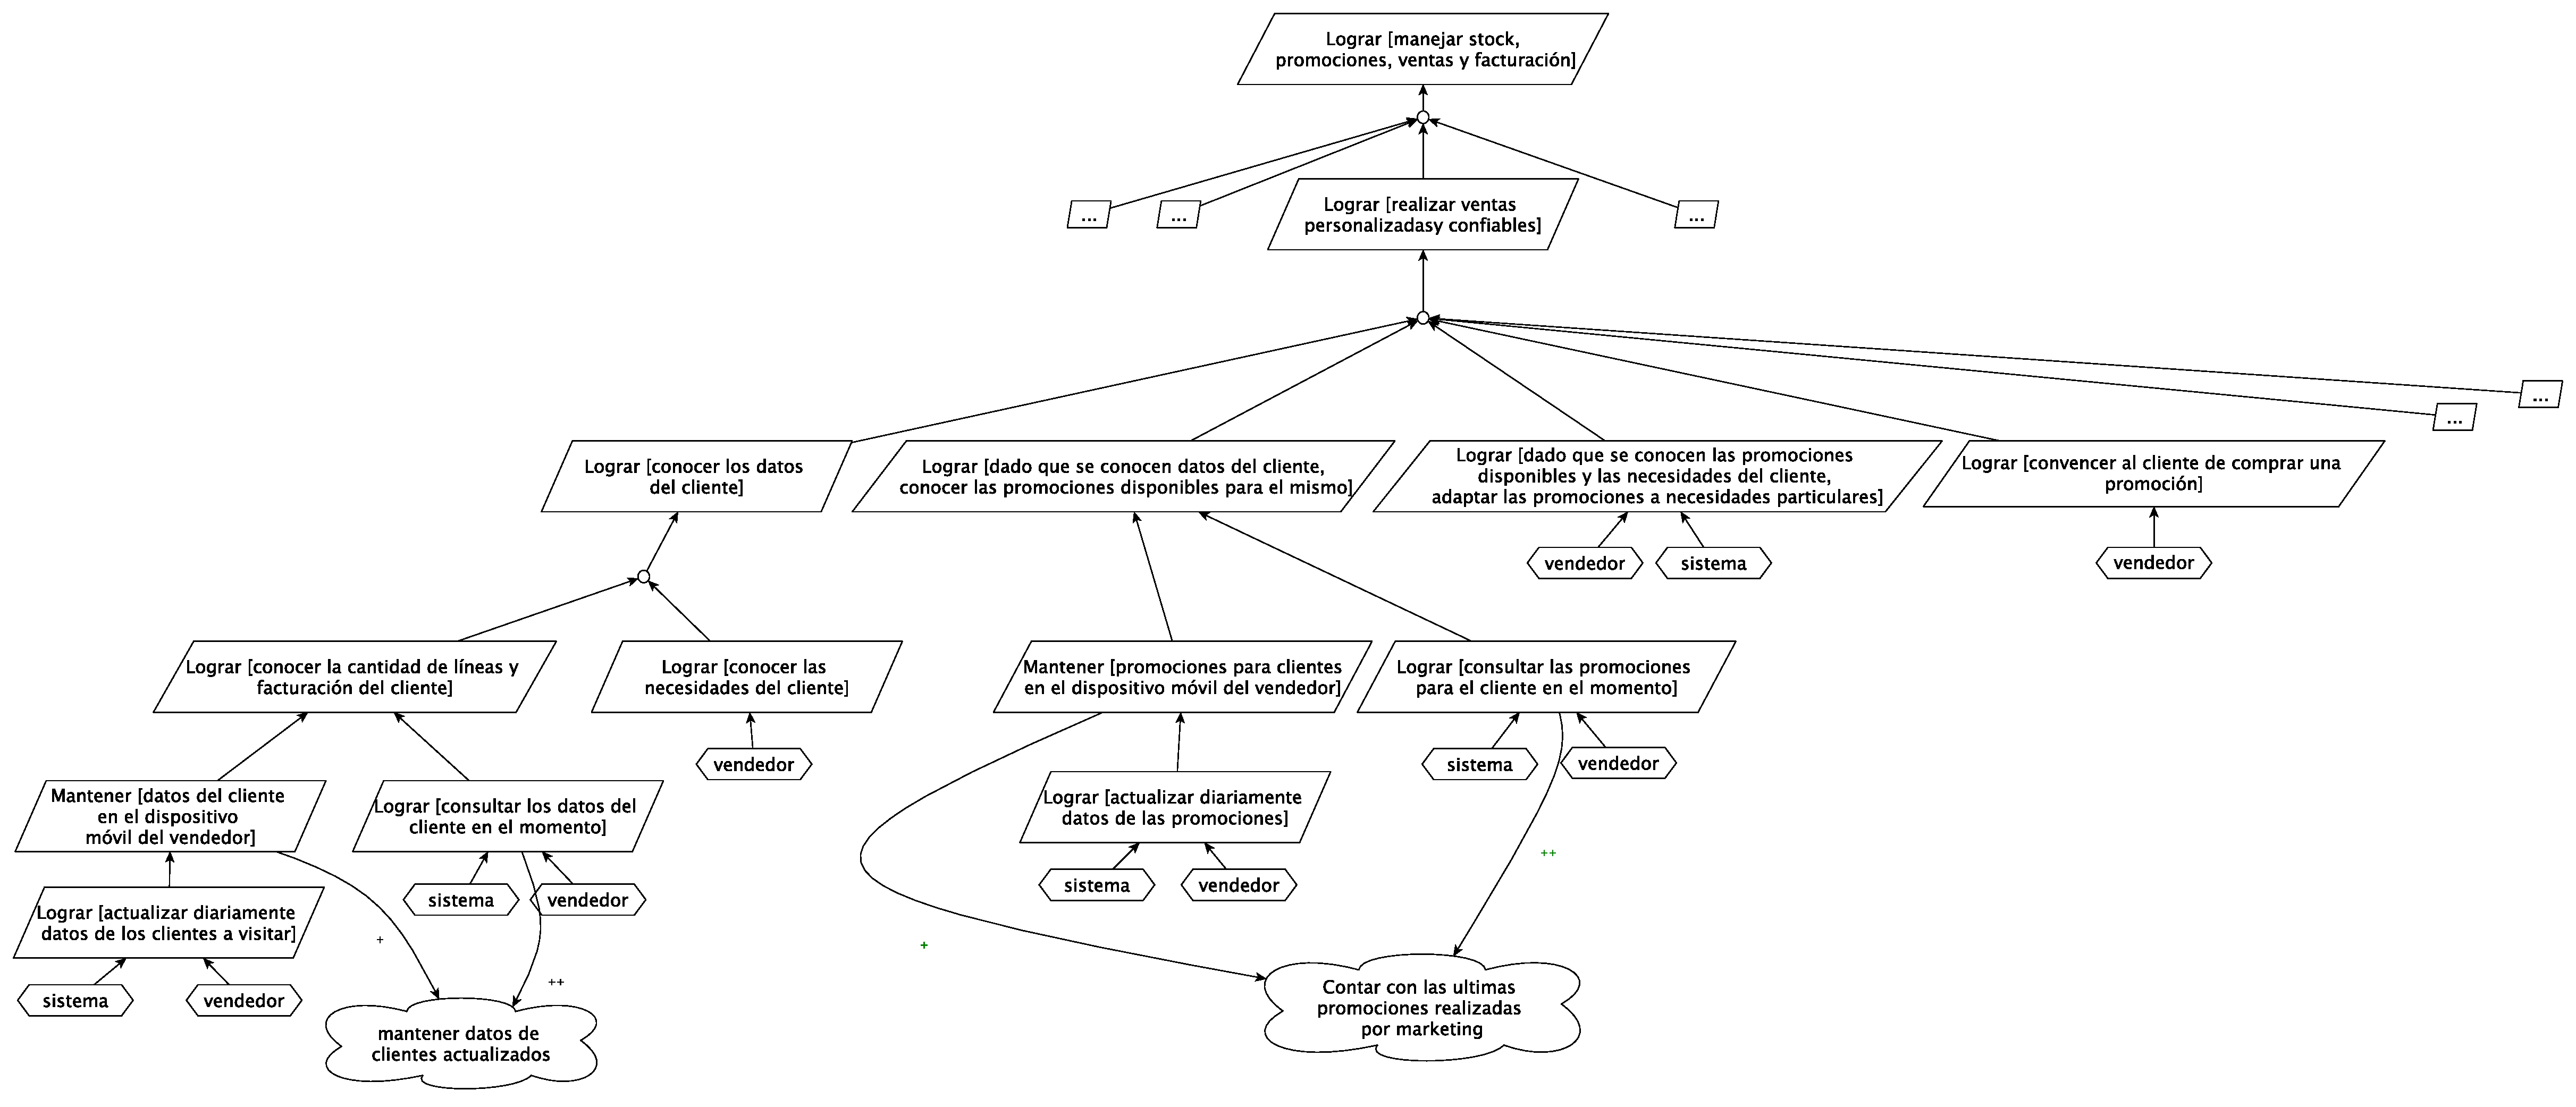
\includegraphics[width=1.5\textwidth, angle=90]{./imagenes/ventas_1.pdf}
  \caption{Diagrama de objetivos - Ventas (parte 1)}
\end{figure}


\clearpage

\clearpage

\begin{figure}[h!]
  \centering
  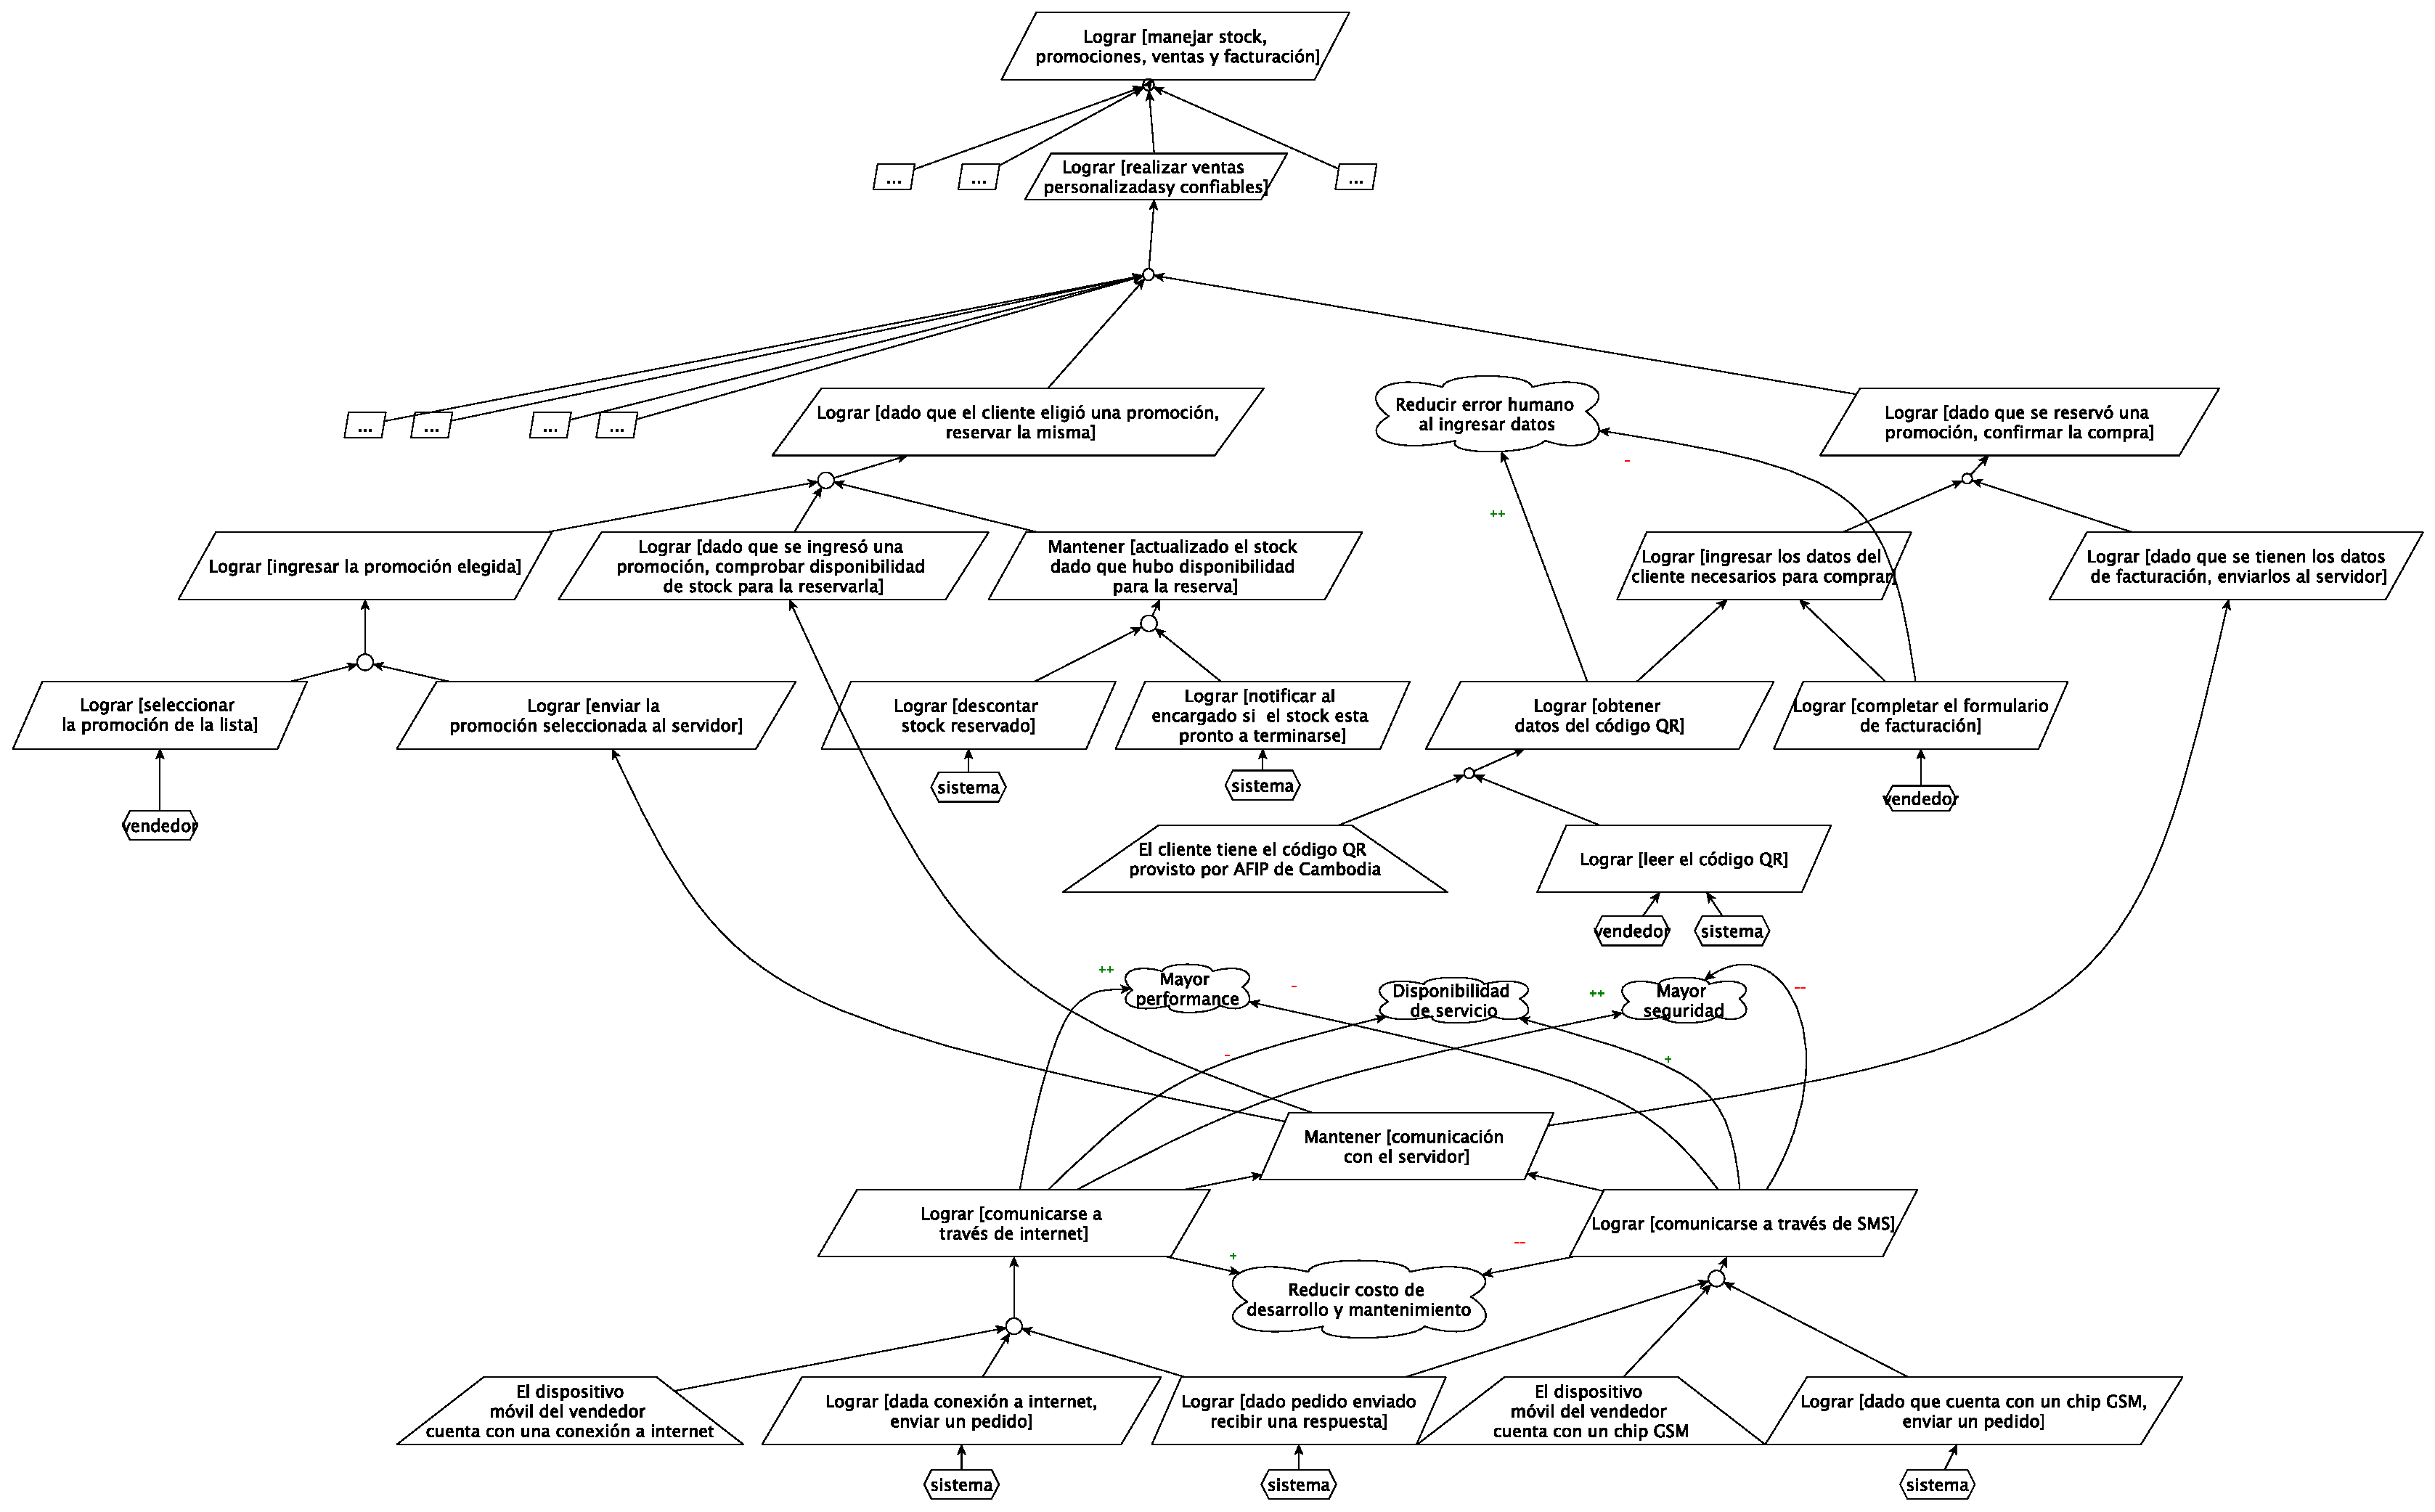
\includegraphics[width=1.5\textwidth, angle=90]{./imagenes/ventas_2.pdf}
  \caption{Diagrama de objetivos - Ventas (parte 2)}
\end{figure}

\clearpage

\subsection{Rama Facturacion}

Finalmente, el último pilar sobre el que se apoya la satisfacción del objetivo principal del sistema es el de facturación. En este aspecto se busca una facturación confiable, lo más automatizada posible a partir de las ventas y que no introduzca errores que enlentezcan el proceso de entrega de equipos a los clientes. Para esto, el departamento de facturación recibe la notificación de las ventas realizadas instantáneamente al haber sido realizadas por los vendedores. Luego, deberá proceder a verificar los datos del cliente y chequear que todo esté en regla, lo cual dependerá explícitamente de los estándares de control implementados por el departamento. Una vez que facturación valide al cliente podrá confirmar la venta a través del sistema, lo cual disparará una notificación al encargado de stock para que se ocupe de armar y coordinar la entrega. Por otro lado, facturación deberá seguir más allá y, utilizando los datos digitalmente provistos por el sistema de ventas, realizar la facturación correspondiente en su sistema externo para tal fin. De cualquier manera se garantizará que haya compatibilidad entre ambos sistemas con el objetivo de que los empleados de facturación no necesiten reingresar ningún dato de manera manual y así poder reducir posibles errores en la etapa final del proceso.

\subsubsection{Escenarios}

\begin{itemize}
  \item \textbf{Confirmar o Rechazar una venta} \\
    Luego que Victor cerró la venta con el cliente, el sistema notifica al departamento de Facturación para proceder con la verificación del estado del Cliente. 
    Fernando, del departamento de facturación verifica que el cliente sea apto 
    para realizar negocios con él bajo el protocolo que corresponda (Veraz, AFIP de Cambodia, etc) 
    y luego utilza nuestro sistema para realizar una de dos acciones:
  \begin{itemize}
    \item \textbf{Confirmar venta de cliente verificado} \\
      Confirma la venta en el sistema que notifica inmediatamente al encargado de Stock que los equipos pueden ser retirados.
    \item \textbf{Rechazar venta de cliente verificado} \\
      Rechaza la venta en el sistema que notifica inmediatamente al encargado de Stock que los equipos no deben ser retirados hasta que no se solucione el problema o vuelvan a estar disponibles.
  \end{itemize}

  \item \textbf{Facturar los equipos y líneas} \\
    Fernando selecciona las ventas confirmadas a facturar y las exporta en un formato compatible con el sistema de Facturación. La integración entre estos sistemas optimiza el tiempo de Fernando y reduce los errores que éste podría cometer.
\end{itemize}

\begin{figure}[h!]
  \centering
  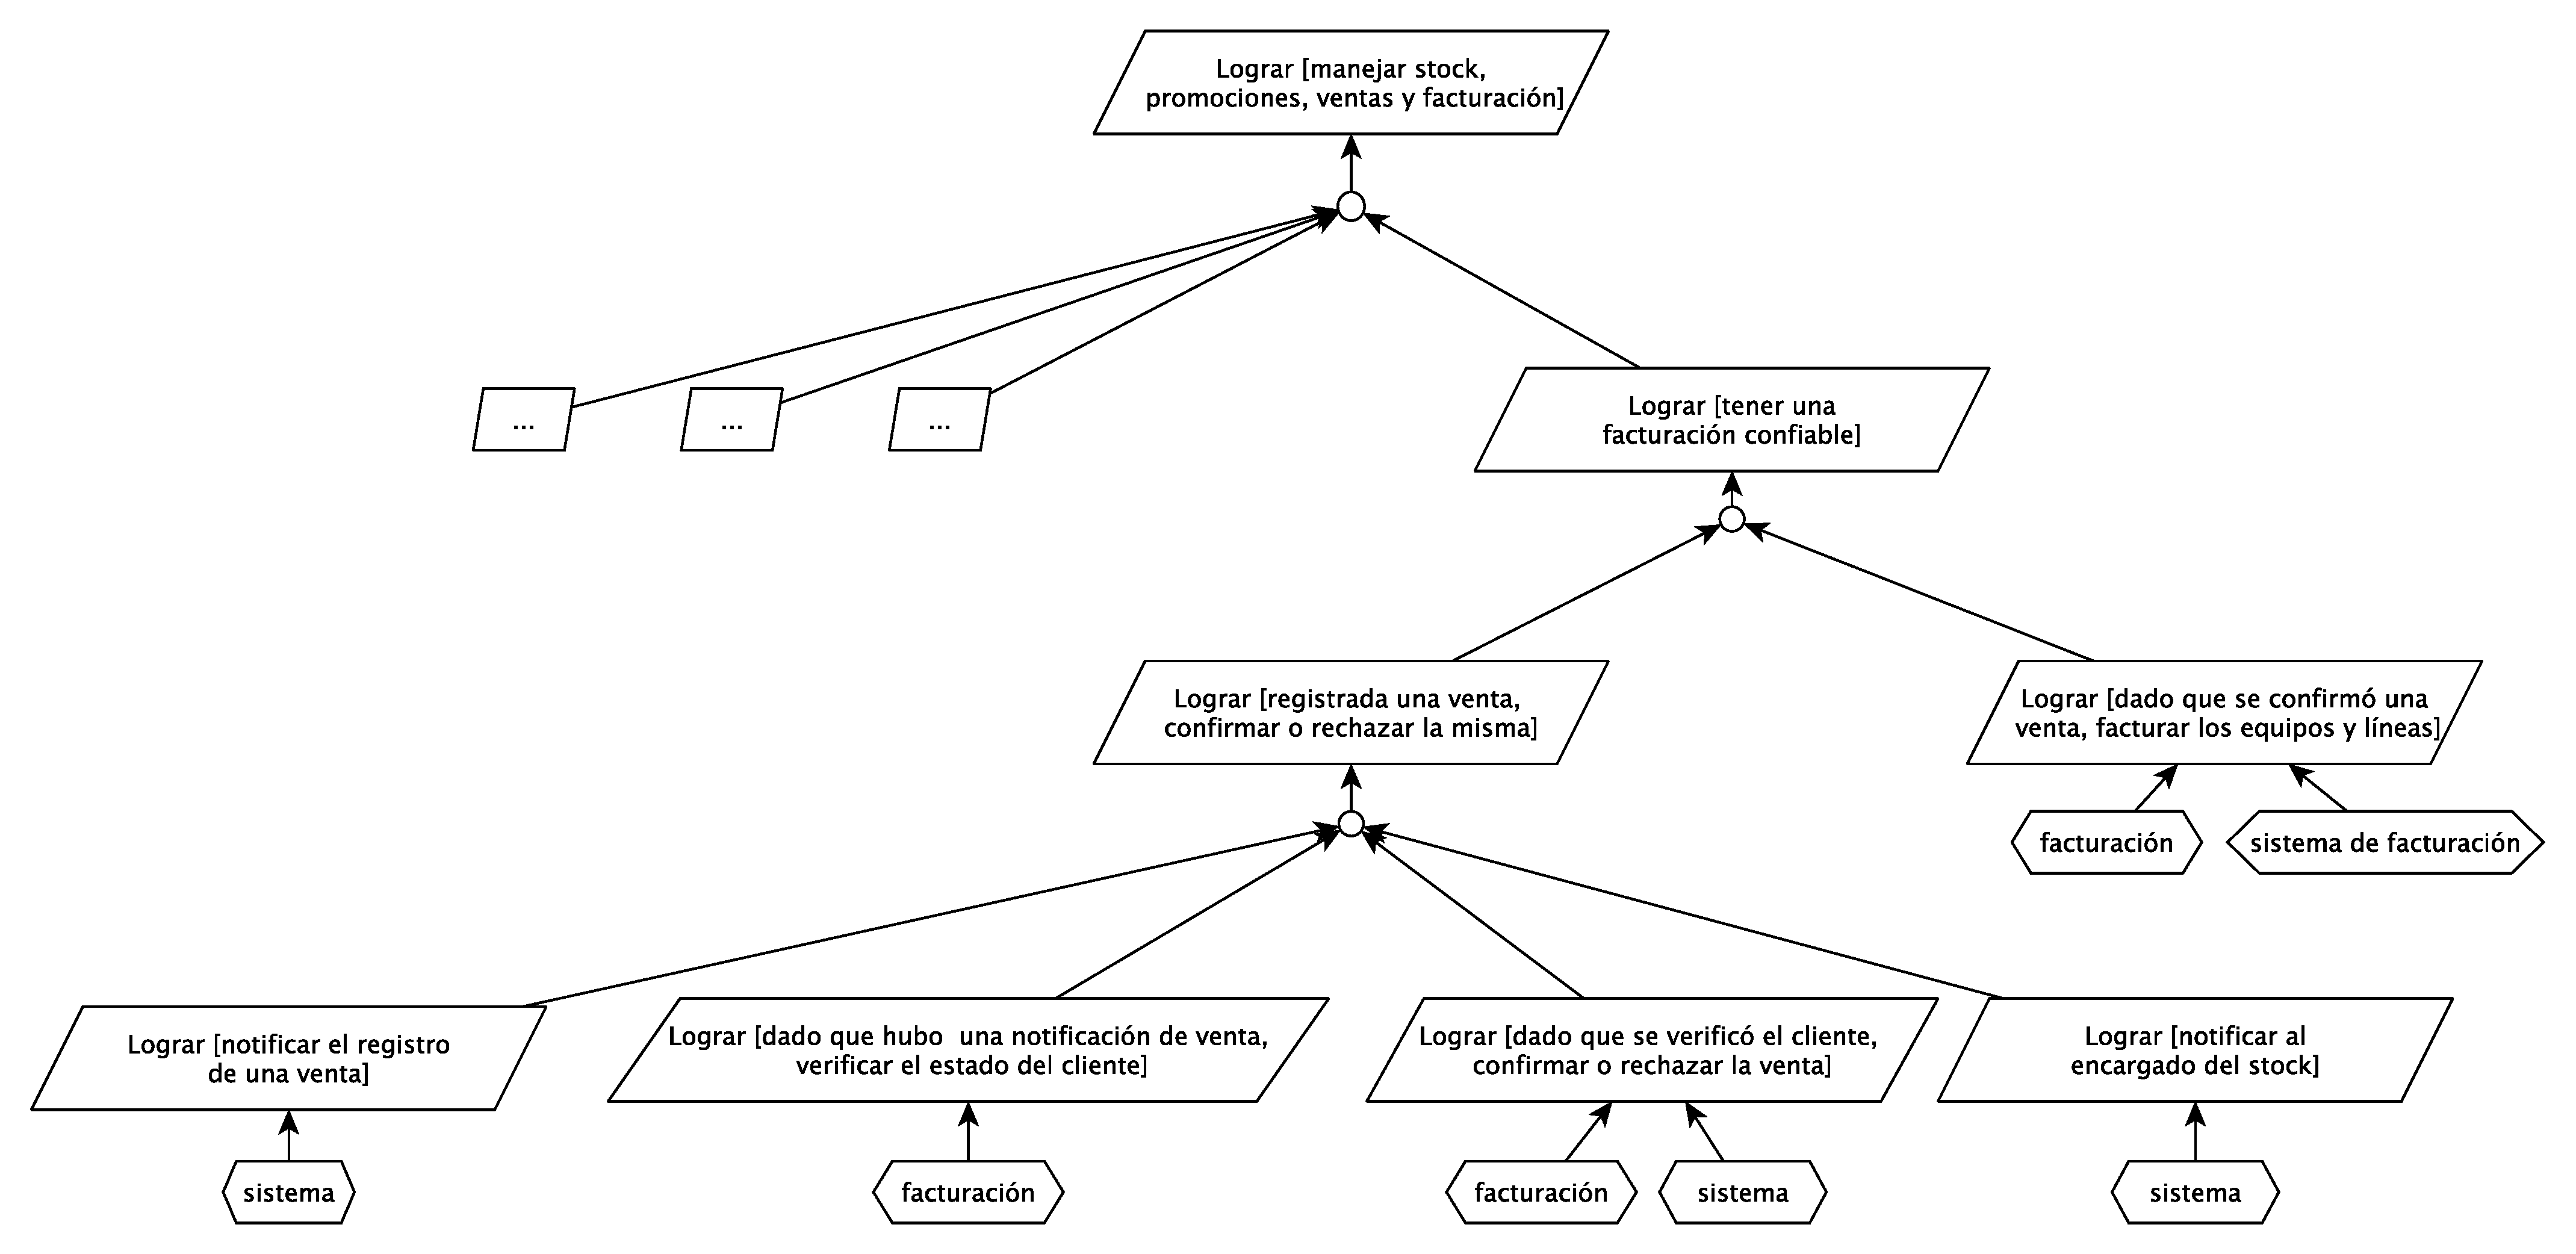
\includegraphics[width=1\textwidth]{./imagenes/facturacion.pdf}
  \caption{Diagrama de objetivos - Facturacion}
\end{figure}

